\documentclass[conference]{IEEEtran}
\IEEEoverridecommandlockouts

\usepackage[utf8]{inputenc}
\usepackage[T1]{fontenc}
\renewcommand{\ttdefault}{lmtt}
\usepackage[spanish,es-nodecimaldot,es-tabla,es-noshorthands]{babel}
\usepackage{cite}
\usepackage{amsmath,amssymb,amsfonts}
\usepackage{bm}
\usepackage{graphicx}
\usepackage{booktabs}
\usepackage{array}
\usepackage{tabularx}
\usepackage{xcolor}
\usepackage{textcomp}
\usepackage{microtype}
\usepackage[hidelinks]{hyperref}

\newcommand{\vect}[1]{\bm{#1}}
\newcommand{\T}{^{\mathsf{T}}}
\newcommand{\sk}[1]{[#1]_{\times}}
\graphicspath{{figs/}{../desarrollo_matematico/figs/}}
\renewcommand{\IEEEkeywordsname}{Palabras clave}
% \input primitivo (expandible) para filas de tablas generadas por scripts/generar_figuras_informe.py
\makeatletter
\newcommand{\tabinput}[1]{\@@input #1 }
\makeatother
% Generado por scripts/generar_datos_calculo.py; no editar a mano
\newcommand{\Ts}{2}
\newcommand{\Fmax}{50}
\newcommand{\Fzero}{4.779}
\newcommand{\MzeroMat}{2.7802 & 0 & 0 & 0 & -0.0003 & 0 \\ 0 & 2.7802 & 0 & 0.0003 & 0 & 0 \\ 0 & 0 & 2.7261 & 0 & 0 & 0 \\ 0 & 0.0003 & 0 & 0.0169 & 0 & 0 \\ -0.0003 & 0 & 0 & 0 & 0.0169 & 0 \\ 0 & 0 & 0 & 0 & 0 & 0.0346}
\newcommand{\MzeroEigs}{0.0169,\allowbreak\ 0.0169,\allowbreak\ 0.0346,\allowbreak\ 2.7261,\allowbreak\ 2.7802,\allowbreak\ 2.7802}
\newcommand{\MzeroEigMin}{0.0169}
\newcommand{\AtwoOneMat}{41.00 & 0 & 0 & 0 & -0.23 & 0 \\ 0 & 41.00 & 0 & 0.23 & 0 & 0 \\ 0 & 0 & 5.74 & 0 & 0 & 0 \\ 0 & 37.89 & 0 & 17.22 & 0 & 0 \\ -37.89 & 0 & 0 & 0 & 17.22 & 0 \\ 0 & 0 & 0 & 0 & 0 & 58.09}
\newcommand{\BtwoMat}{-0.097 & -0.097 & 0.097 & 0 & 0 & 0.097 \\ -0.056 & 0.056 & -0.056 & -0.111 & 0.111 & 0.056 \\ 0.349 & 0.349 & 0.349 & 0.349 & 0.349 & 0.349 \\ -4.966 & 4.966 & 6.786 & 1.820 & -1.820 & -6.786 \\ -4.969 & -4.969 & -1.816 & 6.785 & 6.785 & -1.816 \\ -1.080 & 1.080 & -1.080 & 1.080 & -1.080 & 1.080}
\newcommand{\PolosLA}{\pm7.62,\allowbreak\ \pm6.43\ (\times2),\allowbreak\ \pm4.11\ (\times2),\allowbreak\ \pm2.40}
\newcommand{\SigmaMax}{7.62}
\newcommand{\EigAtwoOne}{58.09,\allowbreak\ 41.36,\allowbreak\ 41.36,\allowbreak\ 16.85,\allowbreak\ 16.85,\allowbreak\ 5.74}
\newcommand{\LamEigs}{0.398,\allowbreak\ 0.398,\allowbreak\ 0.502,\allowbreak\ 4.124,\allowbreak\ 10.371,\allowbreak\ 10.371}
\newcommand{\KlEigs}{427.8,\allowbreak\ 427.8,\allowbreak\ 239.6,\allowbreak\ 6.7,\allowbreak\ 6.7,\allowbreak\ 2.9}
\newcommand{\KlMax}{427.8}
\newcommand{\mLeg}{4.3607}
\newcommand{\kLeg}{185.26}
\newcommand{\mEff}{0.8054}
\newcommand{\sigmaLeg}{6.518}
\newcommand{\cLeg}{1.0000850}
\newcommand{\gLeg}{4.5865\times10^{-7}}
\newcommand{\zUnst}{1.013121}
\newcommand{\zSt}{0.987049}
\newcommand{\MxTheta}{2.94\times10^{-4}}
\newcommand{\muMulti}{1.84\times10^{-6}}
\newcommand{\omegaMulti}{1.9986,\allowbreak\ 1.9986,\allowbreak\ 2.0000,\allowbreak\ 2.0000,\allowbreak\ 2.0014,\allowbreak\ 2.0014}
\newcommand{\MdiagPlat}{2 & 2 & 2 & 0.01125 & 0.01125 & 0.0225}
\newcommand{\MdiagPatas}{0.7802 & 0.7802 & 0.7261 & 0.0057 & 0.0057 & 0.0121}
\newcommand{\KpOpt}{4556.7}
\newcommand{\KiOpt}{18445.7}
\newcommand{\KdOpt}{105.43}
\newcommand{\spOpt}{0.759}
\newcommand{\siOpt}{3.074}
\newcommand{\sdOpt}{0.703}
\newcommand{\TiOpt}{0.247}
\newcommand{\TdOpt}{23.14}
\newcommand{\JpidOpt}{4.777}
\newcommand{\alphaD}{0.7261}
\newcommand{\Dcoef}{136.93}
\newcommand{\nTwo}{18992.4}
\newcommand{\nOne}{-36700.1}
\newcommand{\nZero}{17717.8}
\newcommand{\wcPid}{187.9}
\newcommand{\PMPid}{41.6}
\newcommand{\GMPid}{11.1}
\newcommand{\MsPid}{2.15}
\newcommand{\wcHand}{37.6}
\newcommand{\GwcMag}{1.577\times10^{-4}}
\newcommand{\GwcAng}{-182.2}
\newcommand{\CwcMag}{6343}
\newcommand{\CwcAng}{+31.0}
\newcommand{\PMhand}{28.8}
\newcommand{\RouthA}{105.43}
\newcommand{\RouthB}{4371.4}
\newcommand{\RouthC}{18445.7}
\newcommand{\RouthL}{460870}
\newcommand{\RouthR}{80437}
\newcommand{\RootsCont}{-9.77 \pm 28.57j,\allowbreak\ -4.64}
\newcommand{\charPoly}{z^4 -3.7176z^3 +5.1706z^2 -3.1873z +0.7343}
\newcommand{\charRoots}{0.9907,\allowbreak\ 0.9759 \pm 0.0620j,\allowbreak\ 0.7751}
\newcommand{\rhoSiso}{0.9907}
\newcommand{\rhoPid}{0.9945}
\newcommand{\KpBase}{6000}
\newcommand{\KiBase}{6000}
\newcommand{\KdBase}{150}
\newcommand{\alphaOpt}{3.357}
\newcommand{\betaOpt}{0.3525}
\newcommand{\JssOpt}{3.633}
\newcommand{\PoloCtrl}{-85.60 \pm 30.21j}
\newcommand{\PoloObs}{-27.49 \pm 6.34j}
\newcommand{\tsCtrl}{47}
\newcommand{\cofErr}{2.2\times10^{-16}}
\newcommand{\sepErr}{1.3\times10^{-13}}
\newcommand{\normK}{8.75\times10^{4}}
\newcommand{\rhoSS}{0.9696}
\newcommand{\rhoCtrlBlock}{0.9696}
\newcommand{\obsPoleErr}{5.2\times10^{-15}}
\newcommand{\obsZmax}{0.9465}
\newcommand{\LdPos}{0.104 y 0.132}
\newcommand{\LdVel}{1.585 y 2.598}
\newcommand{\aOnda}{2}
\newcommand{\TOnda}{2.5}
\newcommand{\fOnda}{0.2}
\newcommand{\wOnda}{1.2566}
\newcommand{\AOnda}{15}
\newcommand{\rzZero}{15.000}
\newcommand{\kappaOnda}{0.7170}
\newcommand{\EOnda}{6.738\times10^{-3}}
\newcommand{\TPre}{1}
\newcommand{\rzT}{-15.000}
\newcommand{\drzZero}{0.000}
\newcommand{\drzT}{0.000}
\newcommand{\CUnoA}{-10.8273}
\newcommand{\CDosA}{10.8273}
\newcommand{\xZeroA}{0.000}
\newcommand{\xTA}{0.000}
\newcommand{\JA}{393.7}
\newcommand{\CUnoB}{-10.7539}
\newcommand{\CDosB}{-0.0725}
\newcommand{\xZeroB}{0.000}
\newcommand{\xTB}{-10.899}
\newcommand{\JB}{274.9}
\newcommand{\CUnoC}{0.0725}
\newcommand{\CDosC}{10.7539}
\newcommand{\xZeroC}{10.899}
\newcommand{\xTC}{0.000}
\newcommand{\JC}{274.9}
\newcommand{\CUnoD}{0.0000}
\newcommand{\CDosD}{0.0000}
\newcommand{\xZeroD}{10.754}
\newcommand{\xTD}{-10.754}
\newcommand{\JD}{159.2}
\newcommand{\dlEn}{14.26}
\newcommand{\uEnMax}{17.23}
\newcommand{\EEn}{1.980\times10^{-4}}
\newcommand{\aMax}{0.08}
\newcommand{\dlTm}{23.19}
\newcommand{\TMin}{1.077}
\newcommand{\tSw}{0.538}
\newcommand{\vPico}{43.1}
\newcommand{\uBang}{64.4}
\newcommand{\VAFunoMedia}{-306.92}
\newcommand{\FITunoMedia}{-99.7}
\newcommand{\VAFdosMedia}{97.81}
\newcommand{\FITdosMedia}{84.8}
\newcommand{\FITdosMin}{80.2}
\newcommand{\FITanMedia}{84.7}
\newcommand{\IdHval}{0.1}
\newcommand{\aIdMin}{1.91977}
\newcommand{\aIdMax}{1.99607}
\newcommand{\aAn}{2.00301}
\newcommand{\mIdMin}{0.835}
\newcommand{\mIdMax}{0.900}
\newcommand{\mAn}{0.805}
\newcommand{\IdKp}{1500}
\newcommand{\IdKd}{60}
\newcommand{\IdLmin}{275.1}
\newcommand{\IdLmax}{291.7}
\newcommand{\IdSigma}{0.05}
\newcommand{\mIdDirMin}{0.105}
\newcommand{\mIdDirMax}{0.142}
\newcommand{\IdTsId}{10}
\newcommand{\IdFc}{20}
\newcommand{\IdD}{5}
\newcommand{\mErrMax}{12}

\newcommand{\RefSendl}{14.26}
\newcommand{\RefSendld}{40.33}
\newcommand{\RefSenqdd}{119.91}
\newcommand{\RefSenFff}{4.88}
\newcommand{\RefSendv}{0.00}
\newcommand{\RefSendq}{0.00}
\newcommand{\RefSenFreg}{8.84}
\newcommand{\RefSenPidRms}{0.116}
\newcommand{\RefSenPidEmax}{0.37}
\newcommand{\RefSenPidFmax}{20.6}
\newcommand{\RefSenSsRms}{0.124}
\newcommand{\RefSenSsEmax}{0.52}
\newcommand{\RefSenSsFmax}{8.8}
\newcommand{\RefSeisdl}{22.97}
\newcommand{\RefSeisdld}{39.41}
\newcommand{\RefSeisqdd}{60.45}
\newcommand{\RefSeisFff}{7.32}
\newcommand{\RefSeisdv}{0.00}
\newcommand{\RefSeisdq}{0.00}
\newcommand{\RefSeisFreg}{10.36}
\newcommand{\RefSeisPidRms}{1.424}
\newcommand{\RefSeisPidEmax}{11.99}
\newcommand{\RefSeisPidFmax}{50.0}
\newcommand{\RefSeisSsRms}{0.497}
\newcommand{\RefSeisSsEmax}{11.96}
\newcommand{\RefSeisSsFmax}{50.0}
\newcommand{\RefCircdl}{11.81}
\newcommand{\RefCircdld}{29.68}
\newcommand{\RefCircqdd}{94.75}
\newcommand{\RefCircFff}{7.05}
\newcommand{\RefCircdv}{0.00}
\newcommand{\RefCircdq}{0.00}
\newcommand{\RefCircFreg}{10.15}
\newcommand{\RefCircPidRms}{1.740}
\newcommand{\RefCircPidEmax}{14.96}
\newcommand{\RefCircPidFmax}{50.0}
\newcommand{\RefCircSsRms}{0.690}
\newcommand{\RefCircSsEmax}{14.96}
\newcommand{\RefCircSsFmax}{50.0}
\newcommand{\RefFAdl}{4.68}
\newcommand{\RefFAdld}{20.16}
\newcommand{\RefFAqdd}{59.14}
\newcommand{\RefFAFff}{4.81}
\newcommand{\RefFAdv}{21.44}
\newcommand{\RefFAdq}{0.00}
\newcommand{\RefFAFreg}{8.71}
\newcommand{\RefFAPidRms}{0.096}
\newcommand{\RefFAPidEmax}{0.32}
\newcommand{\RefFAPidFmax}{20.6}
\newcommand{\RefFASsRms}{0.071}
\newcommand{\RefFASsEmax}{0.32}
\newcommand{\RefFASsFmax}{8.7}
\newcommand{\RefFBdl}{10.36}
\newcommand{\RefFBdld}{21.09}
\newcommand{\RefFBqdd}{59.15}
\newcommand{\RefFBFff}{4.82}
\newcommand{\RefFBdv}{22.48}
\newcommand{\RefFBdq}{0.00}
\newcommand{\RefFBFreg}{8.73}
\newcommand{\RefFBPidRms}{0.097}
\newcommand{\RefFBPidEmax}{0.32}
\newcommand{\RefFBPidFmax}{20.6}
\newcommand{\RefFBSsRms}{0.073}
\newcommand{\RefFBSsEmax}{0.32}
\newcommand{\RefFBSsFmax}{8.7}
\newcommand{\RefFCdl}{10.36}
\newcommand{\RefFCdld}{21.46}
\newcommand{\RefFCqdd}{59.15}
\newcommand{\RefFCFff}{4.82}
\newcommand{\RefFCdv}{22.35}
\newcommand{\RefFCdq}{0.00}
\newcommand{\RefFCFreg}{8.71}
\newcommand{\RefFCPidRms}{0.097}
\newcommand{\RefFCPidEmax}{0.34}
\newcommand{\RefFCPidFmax}{20.6}
\newcommand{\RefFCSsRms}{0.072}
\newcommand{\RefFCSsEmax}{0.33}
\newcommand{\RefFCSsFmax}{8.7}
\newcommand{\RefFDdl}{10.23}
\newcommand{\RefFDdld}{21.18}
\newcommand{\RefFDqdd}{42.66}
\newcommand{\RefFDFff}{4.82}
\newcommand{\RefFDdv}{22.19}
\newcommand{\RefFDdq}{0.00}
\newcommand{\RefFDFreg}{8.73}
\newcommand{\RefFDPidRms}{0.098}
\newcommand{\RefFDPidEmax}{0.34}
\newcommand{\RefFDPidFmax}{20.6}
\newcommand{\RefFDSsRms}{0.073}
\newcommand{\RefFDSsEmax}{0.31}
\newcommand{\RefFDSsFmax}{8.7}
\newcommand{\RefFijdl}{23.19}
\newcommand{\RefFijdld}{46.31}
\newcommand{\RefFijqdd}{361.37}
\newcommand{\RefFijFff}{7.41}
\newcommand{\RefFijdv}{39.00}
\newcommand{\RefFijdq}{0.00}
\newcommand{\RefFijFreg}{11.53}
\newcommand{\RefFijPidRms}{0.333}
\newcommand{\RefFijPidEmax}{1.41}
\newcommand{\RefFijPidFmax}{21.7}
\newcommand{\RefFijSsRms}{0.086}
\newcommand{\RefFijSsEmax}{0.47}
\newcommand{\RefFijSsFmax}{11.5}
\newcommand{\RefTmindl}{23.19}
\newcommand{\RefTmindld}{42.99}
\newcommand{\RefTminqdd}{68.05}
\newcommand{\RefTminFff}{6.84}
\newcommand{\RefTmindv}{0.00}
\newcommand{\RefTmindq}{0.00}
\newcommand{\RefTminFreg}{10.21}
\newcommand{\RefTminPidRms}{0.306}
\newcommand{\RefTminPidEmax}{0.88}
\newcommand{\RefTminPidFmax}{21.6}
\newcommand{\RefTminSsRms}{0.083}
\newcommand{\RefTminSsEmax}{0.22}
\newcommand{\RefTminSsFmax}{10.2}
\newcommand{\RefCurvadl}{14.26}
\newcommand{\RefCurvadld}{40.33}
\newcommand{\RefCurvaqdd}{119.91}
\newcommand{\RefCurvaFff}{4.88}
\newcommand{\RefCurvadv}{34.59}
\newcommand{\RefCurvadq}{19.24}
\newcommand{\RefCurvaFreg}{50.00}
\newcommand{\RefCurvaPidRms}{0.605}
\newcommand{\RefCurvaPidEmax}{19.05}
\newcommand{\RefCurvaPidFmax}{50.0}
\newcommand{\RefCurvaSsRms}{0.634}
\newcommand{\RefCurvaSsEmax}{19.20}
\newcommand{\RefCurvaSsFmax}{50.0}


\begin{document}

\title{Modelado, identificación y control de una plataforma Stewart 6-SPS}

\author{\IEEEauthorblockN{Santiago Alejandro Zúñiga Melo}
\IEEEauthorblockA{\textit{Maestría en Ingeniería Electrónica}\\
\textit{Escuela Colombiana de Ingeniería Julio Garavito}\\
Bogotá, Colombia\\
Estrategias Óptimas de Control --- Prof. Jorge Andrés Puerto Acosta, Ph.D.\\
santiago.zuniga-m@mail.escuelaing.edu.co}}

\maketitle

\begin{abstract}
El proyecto integrador tiene como objetivo diseñar, analizar, implementar y comparar estrategias clásicas, modernas y óptimas de control para la posición y la orientación de una plataforma Stewart 6-SPS accionada por seis actuadores lineales. Esta primera entrega construye la base común de esa comparación. Se deriva la cinemática inversa y diferencial y, mediante el principio de Hamilton extendido con el método del momento generalizado, un modelo dinámico de 13 cuerpos rígidos cuya entrada es la fuerza axial de cada actuador. La linealización analítica en el reposo produce un modelo de 12 estados, controlable y observable, cuyos polos en $\pm7.62$~s$^{-1}$ revelan una inestabilidad en lazo abierto causada por la rigidez geométrica negativa de las patas. El modelo se contrasta con una identificación ARX multivariable en lazo cerrado, que reproduce las masas efectivas dentro del 12~\%. Con el cálculo de variaciones y el principio del mínimo de Pontryagin se obtienen trayectorias de referencia óptimas para cuatro casos del integrando y cuatro tipos de frontera. Se diseñan un PID descentralizado y una realimentación de estados con acción integral y observador de Luenberger, cuyos parámetros se obtienen minimizando un criterio común de error y esfuerzo sobre la planta no lineal. La realimentación de estados reduce entre 2.5 y 3 veces el error en los movimientos acoplados con 40~\% menos esfuerzo, mientras que el PID rechaza mejor las perturbaciones.
\end{abstract}

\begin{IEEEkeywords}
plataforma Stewart, robot paralelo, rigidez geométrica, identificación MIMO, cálculo de variaciones, Pontryagin, PID, asignación de estructura propia, observador de Luenberger.
\end{IEEEkeywords}

% =====================================================================================================
\section{Introducción}

La plataforma Stewart--Gough es el manipulador paralelo de seis grados de libertad más estudiado: seis patas extensibles unen una base fija con una plataforma móvil, lo que da alta rigidez y capacidad de carga a cambio de una cinemática directa sin solución cerrada, un acoplamiento multivariable fuerte y una dinámica no lineal \cite{stewart1965,dasgupta2000,merlet2006}. Sus aplicaciones van desde los simuladores de vuelo hasta el aislamiento de vibraciones y el posicionamiento de precisión.

En el control de estos manipuladores coexisten dos enfoques. El primero controla cada pata por separado con un regulador PID sobre su longitud, que se calcula con la cinemática inversa; es simple y robusto, pero trata el acoplamiento entre patas como una perturbación. El segundo usa el modelo dinámico completo, ya sea por par calculado o por realimentación de estados, y compensa el acoplamiento a cambio de depender de la calidad del modelo \cite{dasgupta2000,merlet2006}. La comparación justa entre ambos exige un mismo modelo, un mismo protocolo de ensayo y un mismo criterio de ajuste.

El objetivo general del proyecto es diseñar, analizar, implementar y comparar estrategias clásicas, modernas y óptimas de control para la posición y la orientación de una plataforma Stewart 6-SPS. Esta primera entrega aporta la base común y las dos primeras estrategias:
\begin{itemize}
\item un modelo dinámico de 13 cuerpos, derivado paso a paso y verificado por conservación de la energía y por identificación experimental;
\item la explicación analítica de la inestabilidad en lazo abierto como rigidez geométrica negativa, y la cota de ganancia que impone a cualquier control por pata;
\item trayectorias de referencia óptimas obtenidas con el cálculo de variaciones y el principio de Pontryagin;
\item un PID descentralizado y una realimentación de estados con observador de Luenberger, ajustados con el mismo criterio y comparados sobre la planta no lineal.
\end{itemize}
Las secciones~\ref{sec:plataforma}--\ref{sec:lineal} desarrollan el modelo; la~\ref{sec:ident}, la identificación; la~\ref{sec:var}, las trayectorias; las~\ref{sec:pid}--\ref{sec:opt}, los controladores y su ajuste; la~\ref{sec:resultados}, los resultados, y la~\ref{sec:discusion}, su discusión.

% =====================================================================================================
\section{Descripción de la plataforma}\label{sec:plataforma}

\subsection{Arquitectura y movilidad}

Cada pata está formada por una rótula en la base, un actuador lineal (cilindro y pistón, junta prismática) y una rótula en la plataforma: arquitectura 6-SPS. Con $n$ cuerpos, $j$ juntas y $f_k$ grados de libertad por junta, el criterio de Grübler--Kutzbach da
\begin{equation}
M = 6(n - j - 1) + \sum_{k=1}^{j}f_k .
\label{eq:grubler}
\end{equation}
Con $n = 1 + 1 + 12 = 14$ (base, plataforma, cilindros y pistones), $j = 18$ (6 prismáticas con $f = 1$ y 12 esféricas con $f = 3$):
\begin{equation*}
M = 6(14 - 18 - 1) + (6\cdot1 + 12\cdot3) = -30 + 42 = 12 .
\end{equation*}
Seis de esos grados son giros propios de cada pata sobre su eje, que no mueven la plataforma; la movilidad efectiva es $12 - 6 = 6$, igual al número de actuadores.

\begin{figure}[t]
\centering
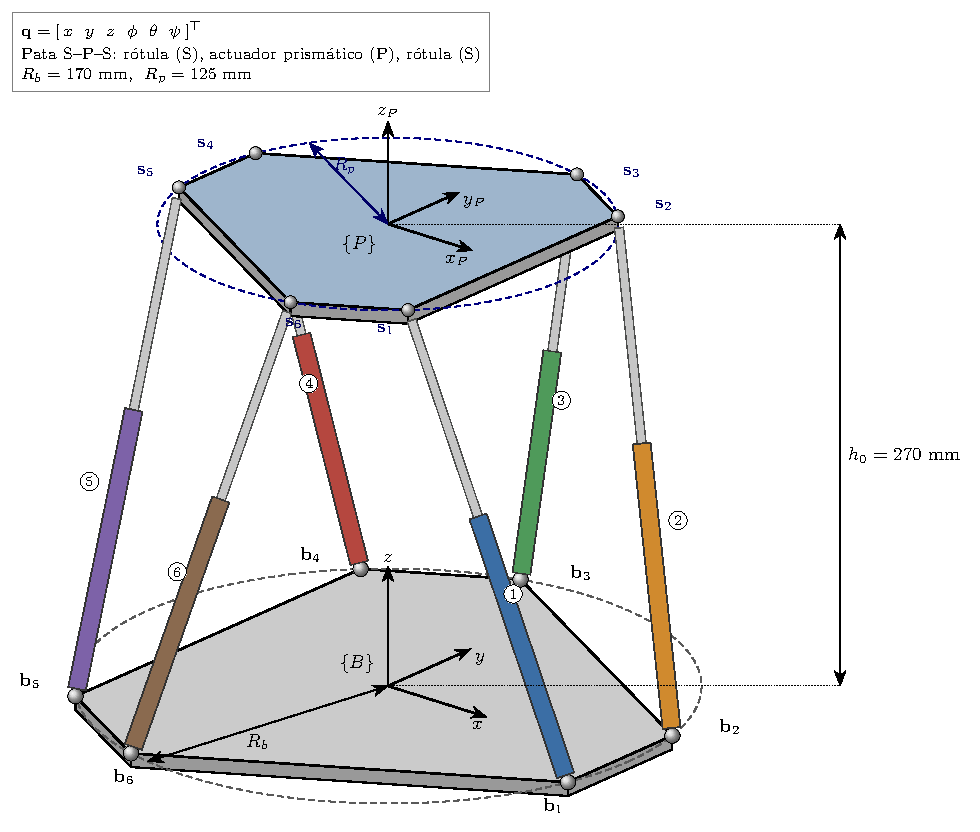
\includegraphics[width=0.8\columnwidth]{arquitectura_6sps.pdf}
\caption{Arquitectura 6-SPS: base $\{B\}$, plataforma $\{P\}$, anclajes $B_i$ y $P_i$ y altura nominal $h_0$.}
\label{fig:arq}
\end{figure}

\subsection{Geometría y parámetros}

Los anclajes están sobre dos circunferencias (Fig.~\ref{fig:geometria}):
\begin{equation}
\vect b_i = R_b\begin{bmatrix}\cos\alpha_{b,i}\\ \sin\alpha_{b,i}\\ 0\end{bmatrix},\qquad
\vect s_i = R_p\begin{bmatrix}\cos\alpha_{p,i}\\ \sin\alpha_{p,i}\\ 0\end{bmatrix},
\end{equation}
con $\alpha_b = \{-15, 15, 105, 135, 225, 255\}^\circ$ y $\alpha_p = \{315, 45, 75, 165, 195, 285\}^\circ$. Cilindro y pistón se modelan como cilindros macizos con el centro de masa en su punto medio:
\begin{equation}
I_\parallel = \tfrac12mr^2,\qquad I_\perp = \tfrac{1}{12}m(3r^2 + L^2),
\end{equation}
lo que da $I_{C,\perp} = 9.762\times10^{-4}$ y $I_{S,\perp} = 1.011\times10^{-4}$~kg\,m$^2$. La plataforma es un disco de radio 150~mm: $\vect I_P = \mathrm{diag}(11.25, 11.25, 22.5)$~g\,m$^2$. La entrada de cada actuador es su fuerza axial $F_i$, con $|F_i| \le \Fmax$~N; se supone que el accionamiento entrega la fuerza comandada. La Tabla~\ref{tab:parametros} resume los parámetros.

\begin{figure}[t]
\centering
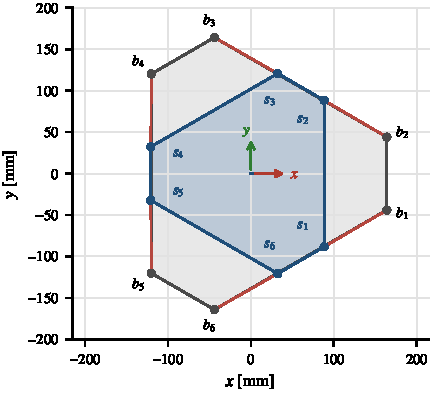
\includegraphics[width=0.75\columnwidth]{geometria.pdf}
\caption{Geometría en la configuración nominal: base (gris), plataforma (azul) y proyección de las patas.}
\label{fig:geometria}
\end{figure}

\begin{table}[t]
\centering
\caption{Parámetros nominales}
\label{tab:parametros}
\scriptsize
\setlength{\tabcolsep}{3pt}
\begin{tabularx}{\columnwidth}{@{}l>{\raggedright\arraybackslash}Xr@{}}
\toprule
Símbolo & Descripción & Valor \\
\midrule
$R_b$ / $R_p$ & Radio de anclajes de la base / plataforma & 170 / 125 mm \\
$h_0$, $l_0$ & Altura nominal, longitud nominal de pata & 270, 283.93 mm \\
$m_P$ & Masa de la plataforma & 2.0 kg \\
$m_C$, $L_C$, $r_C$ & Masa, longitud y radio del cilindro & 0.45 kg, 160, 12 mm \\
$m_S$, $L_S$, $r_S$ & Masa, longitud y radio del pistón & 0.12 kg, 100, 6 mm \\
$b_C$ / $b_S$ & Centro de masa desde $B_i$ / desde $P_i$ & 80 / 50 mm \\
$F_{\max}$ & Fuerza máxima por actuador & $\pm\Fmax$ N \\
$\ddot l_{\max}$ & Aceleración máxima de pata en trayectorias & 0.08 m/s$^2$ \\
$T_s$ & Periodo de muestreo & \Ts{} ms \\
\bottomrule
\end{tabularx}
\end{table}

% =====================================================================================================
\section{Modelo cinemático}\label{sec:cinematica}

\subsection{Orientación y velocidad angular}

Las coordenadas generalizadas son $\vect q = [x\; y\; z\; \phi\; \theta\; \psi]\T$, con la posición $\vect p = [x\; y\; z]\T$ del centro de la plataforma y los ángulos Z--Y--X, $\vect R = \vect R_z(\psi)\vect R_y(\theta)\vect R_x(\phi)$:
\begin{equation}
{\setlength{\arraycolsep}{2pt}\small
\vect R = \begin{bmatrix}
c_\psi c_\theta & c_\psi s_\theta s_\phi - s_\psi c_\phi & c_\psi s_\theta c_\phi + s_\psi s_\phi\\
s_\psi c_\theta & s_\psi s_\theta s_\phi + c_\psi c_\phi & s_\psi s_\theta c_\phi - c_\psi s_\phi\\
-s_\theta & c_\theta s_\phi & c_\theta c_\phi
\end{bmatrix}}.
\end{equation}
Al derivar $\vect R\vect R\T = \vect I$ se obtiene $\dot{\vect R}\vect R\T + \vect R\dot{\vect R}\T = \vect 0$, de modo que $\dot{\vect R}\vect R\T$ es antisimétrica y define la velocidad angular: $\dot{\vect R}\vect R\T = \sk{\vect\omega}$, $\dot{\vect R}\vect s = \vect\omega\times\vect R\vect s$. Derivando el producto de las tres rotaciones y usando $\vect Q\sk{\vect a}\vect Q\T = \sk{\vect Q\vect a}$,
\begin{equation}
\vect\omega = \dot\psi\,\hat{\vect z} + \dot\theta\,\vect R_z\hat{\vect y} + \dot\phi\,\vect R_z\vect R_y\hat{\vect x} = \vect E\dot{\boldsymbol\Theta},
\end{equation}
donde cada término es el eje de giro correspondiente expresado en $\{B\}$: el de guiñada no ha girado, el de cabeceo ya giró con $\vect R_z$ y el de alabeo con $\vect R_z\vect R_y$. Sus columnas son
\begin{equation}
\vect R_z\hat{\vect y} = \begin{bmatrix}-s_\psi\\ c_\psi\\ 0\end{bmatrix},\qquad \vect R_z\vect R_y\hat{\vect x} = \begin{bmatrix}c_\psi c_\theta\\ s_\psi c_\theta\\ -s_\theta\end{bmatrix},
\end{equation}
que forman, junto con $\hat{\vect z}$, las columnas de $\vect E$. Desarrollando el determinante por la última columna, $\det\vect E = c_\psi c_\theta\cdot c_\psi + s_\psi c_\theta\cdot s_\psi = \cos\theta$.
\begin{equation}
\vect E = \begin{bmatrix}c_\psi c_\theta & -s_\psi & 0\\ s_\psi c_\theta & c_\psi & 0\\ -s_\theta & 0 & 1\end{bmatrix},\qquad \det\vect E = \cos\theta ,
\end{equation}
con $\boldsymbol\Theta = [\phi\;\theta\;\psi]\T$. $\vect E$ es invertible para $|\theta| < 90^\circ$; en el espacio de trabajo, $|\theta| \le 18^\circ$ y $\det\vect E \ge 0.951$. La velocidad generalizada (twist) $\vect\nu = [\vect v\T\;\vect\omega\T]\T$ queda
\begin{equation}
\vect\nu = \vect T(\vect q)\,\dot{\vect q},\qquad \vect T = \begin{bmatrix}\vect I_3 & \vect 0\\ \vect 0 & \vect E\end{bmatrix},\qquad \vect T_0 = \vect I_6 .
\label{eq:T}
\end{equation}

\subsection{Cinemática inversa}

El anclaje superior $P_i$ se alcanza por la pata, $\vect b_i + \vect l_i$, o por la plataforma, $\vect p + \vect R\vect s_i$ (Fig.~\ref{fig:lazo}). Igualando ambos caminos se obtiene el lazo vectorial y la longitud de cada pata:
\begin{equation}
\vect l_i = \vect p + \vect R\vect s_i - \vect b_i,\qquad l_i = \lVert\vect l_i\rVert,\qquad \hat{\vect l}_i = \vect l_i/l_i .
\label{eq:ik}
\end{equation}
En el reposo, $\vect p_0 = (0, 0, 270)$~mm y $\vect R = \vect I$; las seis patas miden $l_0 = 283.93$~mm, con $\hat l_{i,z} = 270/283.93 = 0.9509$, y la pata 1 tiene $\hat{\vect l}_1 = (-0.2670, -0.1563, 0.9509)$. La cinemática inversa~\eqref{eq:ik} es la que usan la simulación, el PID y la identificación.

\begin{figure}[t]
\centering
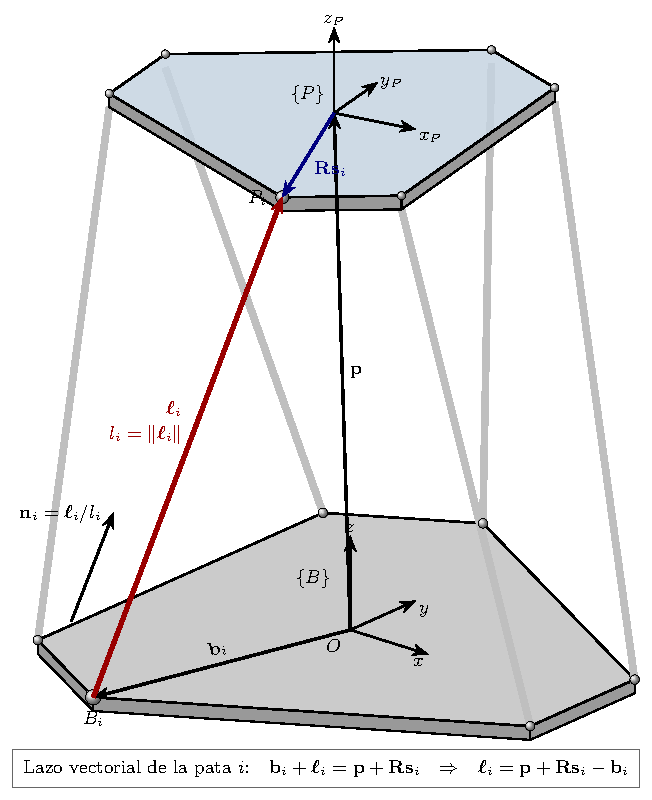
\includegraphics[width=0.62\columnwidth]{lazo_vectorial_pata.pdf}
\caption{Lazo vectorial de la pata $i$: $\vect b_i + \vect l_i = \vect p + \vect R\vect s_i$.}
\label{fig:lazo}
\end{figure}

\subsection{Jacobiano y dualidad estática}

Al derivar $l_i^2 = \vect l_i\T\vect l_i$ se obtiene $l_i\dot l_i = \vect l_i\T\dot{\vect l}_i$, es decir, $\dot l_i = \hat{\vect l}_i\T\dot{\vect l}_i$. Derivando~\eqref{eq:ik} con $\vect p_i = \vect R\vect s_i$:
\begin{equation}
\dot{\vect l}_i = \vect v + \vect\omega\times\vect p_i = \underbrace{\begin{bmatrix}\vect I_3 & \sk{\vect p_i}\T\end{bmatrix}}_{\vect A_i}\vect\nu .
\label{eq:Ai}
\end{equation}
Proyectando sobre la pata y usando la rotación cíclica del triple producto, $\hat{\vect l}_i\cdot(\vect\omega\times\vect p_i) = \vect\omega\cdot(\vect p_i\times\hat{\vect l}_i)$:
\begin{equation}
\dot{\vect l} = \vect J\vect\nu = \vect J\vect T\dot{\vect q},\qquad \vect J_i = \hat{\vect l}_i\T\vect A_i = \begin{bmatrix}\hat{\vect l}_i\T & (\vect p_i\times\hat{\vect l}_i)\T\end{bmatrix}.
\label{eq:jac}
\end{equation}
En el reposo, con la parte angular en metros,
\begin{equation}
{\setlength{\arraycolsep}{1.6pt}\scriptsize
\vect J_0 = \begin{bmatrix}
-0.2670 & -0.1563 & 0.9509 & -0.0841 & -0.0841 & -0.0374\\
-0.2670 & 0.1563 & 0.9509 & 0.0841 & -0.0841 & 0.0374\\
0.2689 & -0.1531 & 0.9509 & 0.1148 & -0.0308 & -0.0374\\
-0.0019 & -0.3094 & 0.9509 & 0.0308 & 0.1148 & 0.0374\\
-0.0019 & 0.3094 & 0.9509 & -0.0308 & 0.1148 & -0.0374\\
0.2689 & 0.1531 & 0.9509 & -0.1148 & -0.0308 & 0.0374
\end{bmatrix}},
\end{equation}
con $\vect p_i = \vect s_i = (s_x, s_y, 0)$ en el reposo, la parte angular de cada fila es $\vect p_i\times\hat{\vect l}_i = (s_y\hat l_z,\ -s_x\hat l_z,\ s_x\hat l_y - s_y\hat l_x)$; para la pata 1, $(-0.08839\cdot0.9509,\ -0.08839\cdot0.9509,\ 0.08839\cdot(-0.1563) + 0.08839\cdot(-0.2670))$ en metros, que es la primera fila de $\vect J_0$. Sus valores singulares son $\{2.329,\allowbreak\ 0.539,\allowbreak\ 0.539,\allowbreak\ 0.198,\allowbreak\ 0.198,\allowbreak\ 0.092\}$ y número de condición $\kappa = 2.329/0.092 = 25.4$. El valor máximo coincide con la norma de la columna vertical, $\sqrt{6}\cdot0.9509 = 2.329$: la dirección vertical es la mejor condicionada, porque las seis patas casi verticales la empujan juntas, y la peor es un giro. En el espacio de trabajo ($\pm45$~mm en $x$--$y$, $\pm18^\circ$ en alabeo y cabeceo), $\kappa \le 27.4$, lejos de las singularidades.

\begin{figure}[t]
\centering
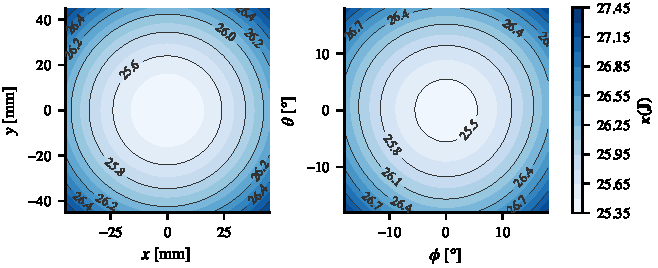
\includegraphics[width=\columnwidth]{condicion_jacobiano.pdf}
\caption{Número de condición $\kappa(\vect J)$ en el espacio de trabajo: traslación horizontal (izquierda) y giros de alabeo y cabeceo (derecha).}
\label{fig:kappa}
\end{figure}

La igualdad de potencias entre las patas y la plataforma, $\vect w\T\vect\nu = \vect F\T\dot{\vect l} = \vect F\T\vect J\vect\nu$ para todo $\vect\nu$, da la dualidad estática
\begin{equation}
\vect w = \vect J\T\vect F,\qquad \vect f_q = (\vect J\vect T)\T\vect F ,
\label{eq:dual}
\end{equation}
donde $\vect w$ son la fuerza y el momento sobre la plataforma y $\vect f_q$ la fuerza generalizada.

\begin{figure}[t]
\centering
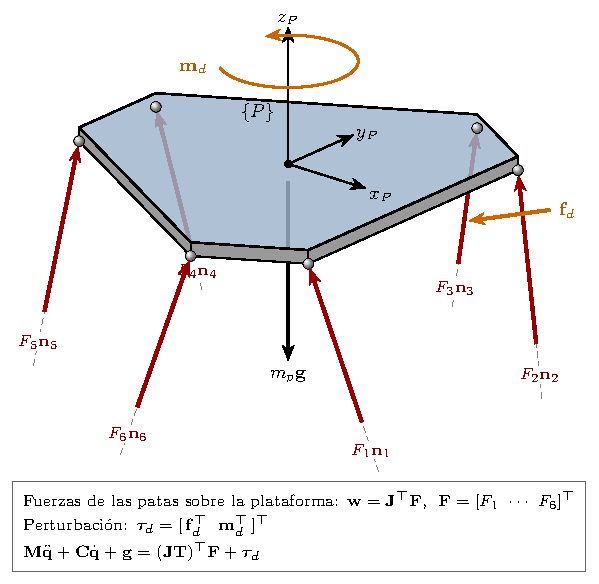
\includegraphics[width=0.85\columnwidth]{cuerpo_libre_plataforma.pdf}
\caption{Diagrama de cuerpo libre de la plataforma: fuerzas axiales de las patas, peso y perturbación; $\vect w = \vect J\T\vect F$.}
\label{fig:dcl}
\end{figure}

\subsection{Velocidad angular de las patas}

Como el giro propio de cada pata no tiene inercia efectiva, su velocidad angular es perpendicular a ella. Derivando $\vect l_i = l_i\hat{\vect l}_i$ se obtiene $\dot{\vect l}_i = \dot l_i\hat{\vect l}_i + \vect\omega_{l_i}\times\vect l_i$; multiplicando vectorialmente por $\vect l_i$ y usando $\vect a\times(\vect b\times\vect c) = (\vect a\cdot\vect c)\vect b - (\vect a\cdot\vect b)\vect c$ con $\vect\omega_{l_i}\perp\vect l_i$:
\begin{equation}
\vect\omega_{l_i} = \frac{\vect l_i\times\dot{\vect l}_i}{\vect l_i\T\vect l_i} = \sk{\bar{\vect l}_i}\vect A_i\vect\nu \equiv \vect J_{D_i}\vect\nu,\qquad \bar{\vect l}_i = \frac{\vect l_i}{l_i^2},
\label{eq:JD}
\end{equation}
y la dirección de la pata cambia como $\dot{\hat{\vect l}}_i = \vect\omega_{l_i}\times\hat{\vect l}_i$.

% =====================================================================================================
\section{Modelo dinámico}\label{sec:dinamica}

\subsection{Velocidades de los centros de masa}

El modelo incluye 13 cuerpos: la plataforma y, en cada pata, el cilindro y el pistón (Fig.~\ref{fig:pata}). Sus centros de masa están en
\begin{equation}
\vect r_P = \vect p,\qquad \vect r_{C_i} = \vect b_i + b_C\hat{\vect l}_i,\qquad \vect r_{S_i} = \vect p + \vect R\vect s_i - b_S\hat{\vect l}_i .
\end{equation}
Derivando con $\dot{\hat{\vect l}}_i = \vect\omega_{l_i}\times\hat{\vect l}_i = \sk{\hat{\vect l}_i}\T\vect\omega_{l_i}$ y con~\eqref{eq:Ai}--\eqref{eq:JD}, cada velocidad queda como una matriz por $\vect\nu$:
\begin{align}
\dot{\vect r}_{C_i} &= b_C\sk{\hat{\vect l}_i}\T\vect J_{D_i}\vect\nu \equiv \vect J_{B_i}\vect\nu, \\
\dot{\vect r}_{S_i} &= \bigl(\vect I_3 - b_S\sk{\hat{\vect l}_i}\T\sk{\bar{\vect l}_i}\bigr)\vect A_i\vect\nu \equiv \vect J_{G_i}\vect\nu ,
\end{align}
y ambos cuerpos giran con $\vect\omega_{l_i} = \vect J_{D_i}\vect\nu$.

\begin{figure}[t]
\centering
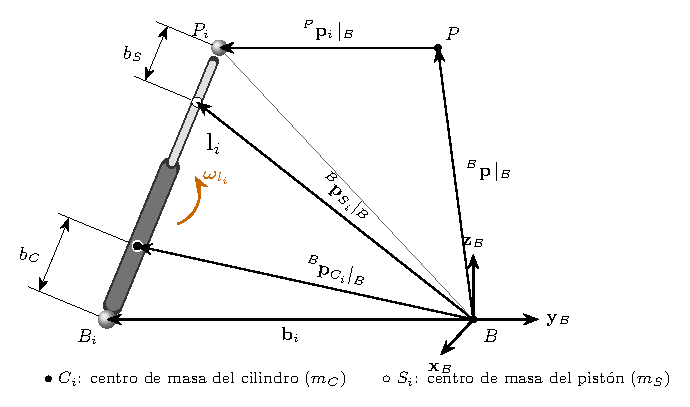
\includegraphics[width=0.85\columnwidth]{cuerpos_pata.pdf}
\caption{Cuerpos de la pata $i$: cilindro con centro de masa a $b_C$ de $B_i$ y pistón con centro de masa a $b_S$ de $P_i$.}
\label{fig:pata}
\end{figure}

\subsection{Energías, trabajo virtual y matriz de inercia}

La energía cinética de un cuerpo es $\frac12m_c\dot{\vect r}_c\T\dot{\vect r}_c + \frac12\vect\omega_c\T\vect I_c|_B\vect\omega_c$, con el tensor llevado a la base, $\vect I_c|_B = \vect R_c\vect I_c|_c\vect R_c\T$. Para una pieza de la pata,
\begin{equation}
\vect I_c|_B = I_\parallel\hat{\vect l}_i\hat{\vect l}_i\T + I_\perp(\vect I - \hat{\vect l}_i\hat{\vect l}_i\T)\ \Rightarrow\ \vect I_c|_B\vect\omega_{l_i} = I_\perp\vect\omega_{l_i},
\end{equation}
porque $\hat{\vect l}_i\T\vect\omega_{l_i} = 0$: solo la inercia transversal interviene. Sumando los 13 cuerpos y sustituyendo $\vect\nu = \vect T\dot{\vect q}$, la energía cinética es $\mathcal T = \frac12\dot{\vect q}\T\vect M(\vect q)\dot{\vect q}$ con
\begin{equation}
\begin{split}
\vect M = \vect T\T\Bigl[&\vect I_P|_B + \textstyle\sum_{i=1}^6\bigl(m_C\vect J_{B_i}\T\vect J_{B_i} + m_S\vect J_{G_i}\T\vect J_{G_i}\\
&+ (I_{C,\perp} + I_{S,\perp})\vect J_{D_i}\T\vect J_{D_i}\bigr)\Bigr]\vect T,
\end{split}
\label{eq:M}
\end{equation}
$\vect I_P|_B = \mathrm{diag}(m_P\vect I_3,\ \vect R\vect I_P\vect R\T)$. Cada sumando tiene la forma $\vect X\T\vect Y\vect X$ con $\vect Y \succeq 0$, de modo que $\vect M = \vect M\T \succ 0$. Esta construcción coincide con la del método del momento generalizado \cite{lopes2009}.

La energía potencial es $\mathcal V = g\bigl(m_Pz + \sum_im_Cz_{C_i} + \sum_im_Sz_{S_i}\bigr)$. Las fuerzas de los actuadores entran por trabajo virtual: con $\delta\vect l = \vect J\vect T\delta\vect q$,
\begin{equation}
\delta W = \vect F\T\delta\vect l + \vect\tau_d\T\delta\vect q = \bigl[(\vect J\vect T)\T\vect F + \vect\tau_d\bigr]\T\delta\vect q \equiv \vect Q\T\delta\vect q ,
\end{equation}
donde $\vect\tau_d$ agrupa las perturbaciones externas.

\subsection{Ecuación de movimiento}

El principio de Hamilton extendido, $\int_{t_0}^{t_f}(\delta L + \vect Q\T\delta\vect q)\,dt = 0$ con $L = \mathcal T - \mathcal V$ y $\delta\vect q(t_0) = \delta\vect q(t_f) = \vect 0$, conduce tras integrar por partes a $\frac{d}{dt}\partial L/\partial\dot{\vect q} - \partial L/\partial\vect q = \vect Q$. Para la componente $i$,
\begin{equation*}
\frac{\partial L}{\partial\dot q_i} = \sum_kM_{ik}\dot q_k,\quad
\frac{d}{dt}\frac{\partial L}{\partial\dot q_i} = \sum_kM_{ik}\ddot q_k + \sum_{j,k}\frac{\partial M_{ik}}{\partial q_j}\dot q_j\dot q_k ,
\end{equation*}
y agrupando los términos de velocidad se obtiene
\begin{equation}
\vect M(\vect q)\ddot{\vect q} + \vect C(\vect q, \dot{\vect q})\dot{\vect q} + \vect g(\vect q) = (\vect J\vect T)\T\vect F + \vect\tau_d ,
\label{eq:dyn}
\end{equation}
\begin{equation}
C_{ik} = \sum_{j=1}^6\Bigl(\frac{\partial M_{ik}}{\partial q_j} - \frac12\frac{\partial M_{jk}}{\partial q_i}\Bigr)\dot q_j,\qquad g_i = \frac{\partial\mathcal V}{\partial q_i}.
\end{equation}
Como la derivada de la posición de cada centro de masa es su Jacobiano de traslación, el vector gravitacional tiene la forma cerrada
\begin{equation}
\vect g = \vect T\T\Bigl(\begin{bmatrix}m_Pg\hat{\vect z}\\ \vect 0\end{bmatrix} + \sum_{i=1}^6\bigl(\vect J_{B_i}\T m_C + \vect J_{G_i}\T m_S\bigr)g\hat{\vect z}\Bigr).
\label{eq:g}
\end{equation}
Con esta definición de $\vect C$ se cumple $\dot{\vect q}\T\vect C\dot{\vect q} = \frac12\dot{\vect q}\T\dot{\vect M}\dot{\vect q}$, y por tanto
\begin{equation}
\frac{d\mathcal T}{dt} = \dot{\vect q}\T(\vect M\ddot{\vect q} + \vect C\dot{\vect q}) = \dot{\vect q}\T(\vect Q - \vect g),
\end{equation}
que es el balance de energía: sin fuerzas ni gravedad, $\mathcal T$ se conserva.

\textbf{Forma de Christoffel y pasividad.} La matriz $\vect C$ no es única: cualquier otra con el mismo producto $\vect C\dot{\vect q}$ describe la misma dinámica. Simetrizando los dos primeros términos de $\frac{d}{dt}\partial L/\partial\dot q_i$ se obtiene la elección de Christoffel,
\begin{equation}
C^{\Gamma}_{ik} = \sum_{j=1}^6c_{ijk}\dot q_j,\quad c_{ijk} = \frac12\Bigl(\frac{\partial M_{ik}}{\partial q_j} + \frac{\partial M_{ij}}{\partial q_k} - \frac{\partial M_{jk}}{\partial q_i}\Bigr),
\label{eq:christoffel}
\end{equation}
con $\vect C^\Gamma\dot{\vect q} = \vect C\dot{\vect q}$ porque $c_{ijk}$ y $c_{ikj}$ se suman igual contra $\dot q_j\dot q_k$. Con esta elección, como $\dot M_{ik} = \sum_j(\partial M_{ik}/\partial q_j)\dot q_j$,
\begin{equation}
\bigl(\dot{\vect M} - 2\vect C^\Gamma\bigr)_{ik} = \sum_{j=1}^6\Bigl(\frac{\partial M_{jk}}{\partial q_i} - \frac{\partial M_{ij}}{\partial q_k}\Bigr)\dot q_j ,
\end{equation}
que cambia de signo al intercambiar $i$ y $k$: $\dot{\vect M} - 2\vect C^\Gamma$ es antisimétrica y $\dot{\vect q}\T(\dot{\vect M} - 2\vect C^\Gamma)\dot{\vect q} = 0$ para todo $\dot{\vect q}$. Con la energía total $\mathcal E = \mathcal T + \mathcal V$ y la fuerza generalizada de~\eqref{eq:dual},
\begin{equation}
\dot{\mathcal E} = \dot{\vect q}\T\bigl[(\vect J\vect T)\T\vect F + \vect\tau_d\bigr] = \dot{\vect l}\T\vect F + \dot{\vect q}\T\vect\tau_d ,
\end{equation}
es decir, el mapa de las fuerzas de los actuadores a las velocidades de las patas es pasivo: la potencia que entra por los actuadores es exactamente la que cambia la energía mecánica. Además, como $\vect M$ es simétrica y definida positiva, en el espacio de trabajo $\lambda_{\min}\lVert\dot{\vect q}\rVert^2 \le 2\mathcal T \le \lambda_{\max}\lVert\dot{\vect q}\rVert^2$, con $\lambda(\vect M_0)\in[\MzeroEigMin,\ 2.7802]$ en el reposo.

Con $\vect x = [\vect q\T\;\dot{\vect q}\T]\T$ y $\vect u = \vect F$, la forma de primer orden es
\begin{equation}
\dot{\vect x} = \begin{bmatrix}\dot{\vect q}\\ \vect M^{-1}\bigl[(\vect J\vect T)\T\vect u + \vect\tau_d - \vect C\dot{\vect q} - \vect g\bigr]\end{bmatrix},\qquad \vect y = \vect q .
\label{eq:fnl}
\end{equation}

\begin{figure}[t]
\centering
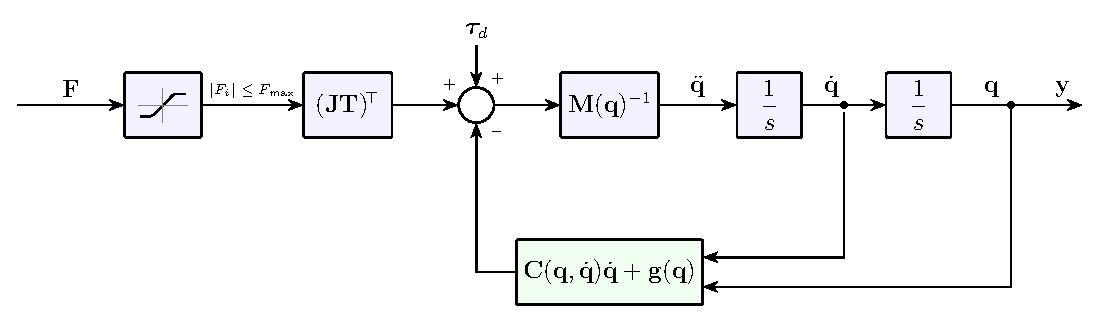
\includegraphics[width=\columnwidth]{diagrama_bloques_dinamico.pdf}
\caption{Diagrama de bloques del modelo dinámico~\eqref{eq:fnl}.}
\label{fig:bloques}
\end{figure}

\subsection{Valores en el reposo y verificación}

En el reposo, $\vect T_0 = \vect I_6$ y la matriz de inercia es
\begin{equation}
{\setlength{\arraycolsep}{2.5pt}\footnotesize
\vect M_0 = \begin{bmatrix}\MzeroMat\end{bmatrix}},
\end{equation}
en kg, kg\,m y kg\,m$^2$. La masa en $x$ e $y$ es $2 + 0.7802 = 2.7802$~kg: las patas aportan el $0.7802/2.7802 = 28$~\% de la inercia de traslación, y un modelo que las omitiera la subestimaría en casi un tercio. Las seis entradas fuera de la diagonal, $M_{x\theta} = -M_{y\phi} = 3\times10^{-4}$~kg\,m, provienen de la asimetría de los pistones.

La única componente no nula de $\vect g_0$ es la vertical, $g_z = m_Pg + 6m_Cg(\vect J_{B_i})_{zz} + 6m_Sg(\vect J_{G_i})_{zz} = 19.613 + 0.715 + 6.942 = 27.270$~N, el 51.3~\% del peso total de 53.15~N; el resto lo soportan las rótulas de la base. En equilibrio, \eqref{eq:dyn} se reduce a $\vect J_0\T\vect F_0 = \vect g_0$; por simetría las seis fuerzas son iguales y, como la suma de la columna vertical de $\vect J_0$ es $6\cdot0.9509 = 5.705$,
\begin{equation}
F_0 = \frac{27.270}{5.705} = \Fzero\ \text{N}.
\end{equation}
El modelo se verificó de tres formas: la energía cinética en movimiento libre se conserva con una deriva relativa de $3.2\times10^{-13}$ en 0.5~s; $\vect g$ de~\eqref{eq:g} coincide con el gradiente numérico de $\mathcal V$ con error menor que $10^{-9}$~N, y la dinámica inversa de una maniobra de prueba da fuerzas entre 3.03 y 6.74~N, coherentes con $F_0$.

\begin{figure}[t]
\centering
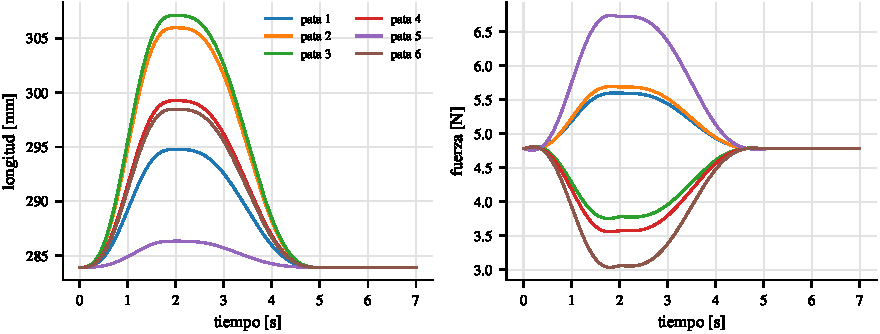
\includegraphics[width=\columnwidth]{validacion_modelo.pdf}
\caption{Dinámica inversa en la maniobra de prueba: longitudes y fuerzas de los seis actuadores calculadas con~\eqref{eq:dyn}.}
\label{fig:valid}
\end{figure}

% =====================================================================================================
\section{Linealización y propiedades estructurales}\label{sec:lineal}

\subsection{Modelo lineal analítico}

Se linealiza~\eqref{eq:fnl} en $\vect x_0 = [0\;0\;h_0\;0\;0\;0\;\vect 0]\T$, $\vect u_0 = F_0\vect 1$. Escribiendo la segunda fila como $\vect M^{-1}\vect h$, con $\vect h = (\vect J\vect T)\T\vect u + \vect\tau_d - \vect C\dot{\vect q} - \vect g$, su derivada respecto a cualquier variable $\xi$ es
\begin{equation}
\frac{\partial(\vect M^{-1}\vect h)}{\partial\xi}\Big|_0 = \frac{\partial\vect M^{-1}}{\partial\xi}\underbrace{\vect h_0}_{\vect 0} + \vect M_0^{-1}\frac{\partial\vect h}{\partial\xi}\Big|_0 ,
\end{equation}
de modo que no hace falta derivar $\vect M^{-1}$. Además $\vect C\dot{\vect q}$ es cuadrático en $\dot{\vect q}$ y su derivada se anula en el reposo. Queda
\begin{equation}
\vect A = \begin{bmatrix}\vect 0 & \vect I_6\\ \vect A_{21} & \vect 0\end{bmatrix},\quad
\vect B = \begin{bmatrix}\vect 0\\ \vect B_2\end{bmatrix},\quad
\vect C_y = \begin{bmatrix}\vect I_6 & \vect 0\end{bmatrix},
\label{eq:AB}
\end{equation}
\begin{equation}
\vect A_{21} = -\vect M_0^{-1}\vect K_q,\qquad \vect B_2 = \vect M_0^{-1}\vect J_0\T,
\end{equation}
donde $\vect K_q = -\partial[(\vect J\vect T)\T\vect u_0 - \vect g]/\partial\vect q|_0$. Como $(\vect J\vect T)\T\vect F_0 = F_0\sum_i\nabla_{\vect q}l_i$ y $\vect g = \nabla_{\vect q}\mathcal V$, la rigidez es una hessiana, y por tanto simétrica:
\begin{equation}
\vect K_q = \underbrace{-F_0\sum_{i=1}^6\nabla^2_{\vect q}l_i}_{\text{precarga}} + \underbrace{\nabla^2_{\vect q}\mathcal V_g}_{\text{peso de las patas}} .
\label{eq:Kq}
\end{equation}
Escribiendo $l_i = \lVert\vect r_i(\vect q) - \vect b_i\rVert$ con $\vect r_i = \vect p + \vect R\vect s_i$ y aplicando la regla de la cadena dos veces,
\begin{equation}
\nabla^2_{\vect q}l_i = \Bigl(\frac{\partial\vect r_i}{\partial\vect q}\Bigr)\T\frac{\vect I_3 - \hat{\vect l}_i\hat{\vect l}_i\T}{l_i}\,\frac{\partial\vect r_i}{\partial\vect q} + \sum_{k=1}^3\hat l_{i,k}\,\nabla^2_{\vect q}r_{i,k},
\label{eq:hesl}
\end{equation}
donde en el reposo $\partial\vect r_i/\partial\vect q = \vect A_i$. El primer término es la rigidez geométrica de la pata, que se analiza en la subsección siguiente; el segundo aparece solo en los giros, porque $\vect r_i$ es lineal en $\vect p$ y no lineal en $\boldsymbol\Theta$. En el bloque de traslación solo queda el primero, y su entrada $xx$ es $-F_0\sum_i(1 - \hat l_{i,x}^2)/l_0 = -4.7795\cdot5.7128/0.28393 = -96.16$~N/m.

Sus entradas diagonales valen $-113.99$~N/m en $x$ e $y$ ($-96.16$ de precarga y $-17.83$ de peso), $-15.65$~N/m en $z$, $-0.29$~N\,m/rad en alabeo y cabeceo y $-2.01$~N\,m/rad en guiñada. Todas son negativas.

\subsection{Rigidez geométrica negativa}

Una pata con fuerza constante $F_0$ tiene la energía $\mathcal V_F = -F_0l_i$. Con $l = \lVert\vect r - \vect b_i\rVert$,
\begin{equation}
\nabla_{\vect r}l = \hat{\vect l}_i,\qquad \nabla^2_{\vect r}l = \frac{1}{l}\bigl(\vect I_3 - \hat{\vect l}_i\hat{\vect l}_i\T\bigr) \succeq 0,
\end{equation}
cuyos valores propios son $0$ en la dirección de la pata y $1/l$ en las dos perpendiculares. La rigidez $-F_0\nabla^2l$ es entonces negativa: cada pata empuja la plataforma lejos del equilibrio con $F_0/l_0 = 4.779/0.28393 = 16.8$~N/m en el plano perpendicular a ella, igual que un péndulo invertido. Con la estructura de~\eqref{eq:AB}, $\vect A\vect w = \lambda\vect w$ implica $\vect w_2 = \lambda\vect w_1$ y $\vect A_{21}\vect w_1 = \lambda^2\vect w_1$; como $\lambda(\vect A_{21}) = \{\EigAtwoOne\}$~s$^{-2}$ es positivo,
\begin{gather}
\lambda(\vect A) = \pm\sqrt{\lambda(\vect A_{21})}\nonumber\\ = \{\PolosLA\}\ \text{s}^{-1}.
\end{gather}
La plataforma es inestable en lazo abierto en los seis grados de libertad. El modo más rápido, la guiñada, duplica una perturbación en $\ln2/7.62 = 91$~ms, 45 veces el periodo de muestreo (Fig.~\ref{fig:polos}).

En las coordenadas de las patas, con $\delta\vect q = \vect J_0^{-1}\delta\vect l$ y multiplicando por $\vect J_0^{-\top}$,
\begin{gather}
\boldsymbol\Lambda\,\delta\ddot{\vect l} = \delta\vect F + \vect K_l\,\delta\vect l, \label{eq:patas}\\
\boldsymbol\Lambda = \vect J_0^{-\top}\vect M_0\vect J_0^{-1},\qquad \vect K_l = \vect J_0^{-\top}\vect K_q^{-}\vect J_0^{-1},\nonumber
\end{gather}
con $\vect K_q^- = -\vect K_q$, $\lambda(\boldsymbol\Lambda) = \{\LamEigs\}$~kg y $\lambda(\vect K_l) = \{\KlEigs\}$~N/m. Con una realimentación proporcional por pata, $\delta\vect F = -K_p\delta\vect l$, la rigidez neta es $K_p\vect I - \vect K_l$, que es definida positiva si y solo si
\begin{equation}
K_p > \lambda_{\max}(\vect K_l) = \KlMax\ \text{N/m}.
\label{eq:cotaKp}
\end{equation}
Esta cota vale para cualquier control descentralizado.

La Fig.~\ref{fig:la} compara la respuesta libre de la planta no lineal~\eqref{eq:fnl} con la del modelo lineal, $\delta\vect x(t) = e^{\vect At}\delta\vect x(0)$, desde una perturbación de 1~mm en $x$ y $0.2^\circ$ en guiñada con $\vect F = \vect F_0$: ambas crecen como $e^{\sigma t}$ y coinciden mientras la perturbación es pequeña, lo que confirma a la vez la inestabilidad y la validez local del modelo lineal. La Fig.~\ref{fig:frec} muestra los valores singulares de $\vect G(j\omega) = \vect C_y(j\omega\vect I - \vect A)^{-1}\vect B$: planos por debajo de los polos inestables, con $\vect G(0) = -\vect C_y\vect A^{-1}\vect B = -\vect A_{21}^{-1}\vect B_2 = \vect K_q^{-1}\vect J_0\T$, y con pendiente de $-40$~dB/década por encima, como un doble integrador con la masa de cada dirección. La curva de una pata, $1/|m(j\omega)^2 - k|$, es la que usa el PID.

\begin{figure}[t]
\centering
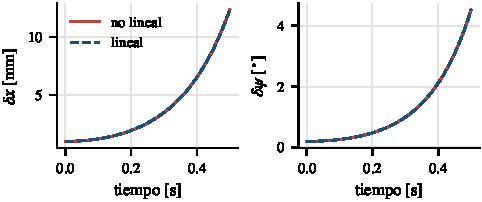
\includegraphics[width=\columnwidth]{modelo_lazo_abierto.pdf}
\caption{Respuesta libre en lazo abierto con $\vect F = \vect F_0$: planta no lineal y modelo lineal.}
\label{fig:la}
\end{figure}

\begin{figure}[t]
\centering
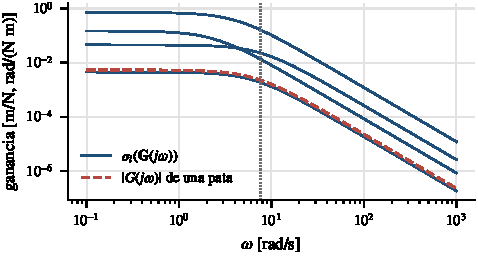
\includegraphics[width=\columnwidth]{modelo_frecuencia.pdf}
\caption{Valores singulares del modelo lineal $\vect G(j\omega)$ y respuesta de una pata. La línea punteada marca $\sigma_{\max} = 7.62$~s$^{-1}$.}
\label{fig:frec}
\end{figure}

\begin{figure}[t]
\centering
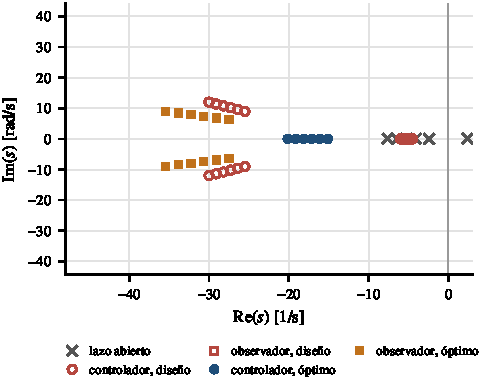
\includegraphics[width=0.9\columnwidth]{polos.pdf}
\caption{Polos del modelo lineal en lazo abierto y en lazo cerrado.}
\label{fig:polos}
\end{figure}

\subsection{Discretización exacta}

Con retenedor de orden cero, $\vect A_d = e^{\vect AT_s}$ y $\vect B_d = \int_0^{T_s}e^{\vect A\eta}d\eta\,\vect B$, ambos obtenidos con una sola exponencial \cite{vanloan1978}. Por la estructura de $\vect A$, $\vect A^{2k} = \mathrm{diag}(\vect A_{21}^k, \vect A_{21}^k)$, y la serie se agrupa en funciones hiperbólicas de $\vect S = \vect A_{21}^{1/2}$:
\begin{gather}
\vect A_d = \begin{bmatrix}\cosh\vect ST_s & \vect S^{-1}\sinh\vect ST_s\\ \vect S\sinh\vect ST_s & \cosh\vect ST_s\end{bmatrix},\nonumber\\
\vect B_d = \begin{bmatrix}\vect A_{21}^{-1}(\cosh\vect ST_s - \vect I)\vect B_2\\ \vect S^{-1}\sinh(\vect ST_s)\vect B_2\end{bmatrix}.
\end{gather}
La segunda forma sale de integrar término a término: $\int_0^{T_s}\cosh(\vect S\eta)\,d\eta = \vect S^{-1}\sinh\vect ST_s$ y $\int_0^{T_s}\vect S^{-1}\sinh(\vect S\eta)\,d\eta = \vect S^{-2}(\cosh\vect ST_s - \vect I)$, con $\vect S^{-2} = \vect A_{21}^{-1}$; como $\vect B$ solo tiene el bloque inferior, $\vect B_d$ toma la segunda columna de bloques. Para $T_s$ pequeño, $\vect A_d \approx \vect I + \vect AT_s$ y $\vect B_d \approx [\frac12T_s^2\vect B_2;\ T_s\vect B_2]$: la fuerza entra en la posición con un factor $T_s^2/2$ y en la velocidad con $T_s$. Cada polo pasa a $z = e^{\lambda T_s}$; el más inestable queda en $e^{0.01524} = 1.0154$, fuera del círculo unitario. Con $T_s = 2$~ms, $\lVert\vect A_{21}\rVert T_s^2 \approx 2\times10^{-4}$.

\subsection{Controlabilidad, observabilidad y ceros}

Como $\vect C_y\vect A = [\vect 0\;\vect I_6]$, la matriz de observabilidad contiene $\mathrm{diag}(\vect I_6, \vect I_6) = \vect I_{12}$: midiendo $\vect q$ se reconstruyen las velocidades. Como $\vect A\vect B = [\vect B_2\T\;\vect 0]\T$,
\begin{equation}
\begin{split}
\det\begin{bmatrix}\vect B & \vect A\vect B\end{bmatrix} &= \det(\vect B_2)^2 = \Bigl(\frac{\det\vect J_0}{\det\vect M_0}\Bigr)^2\\ &= (-11.64)^2 \ne 0,
\end{split}
\end{equation}
y el sistema es controlable con las seis fuerzas mientras $\vect J_0$ no sea singular. Por último, la matriz de Rosenbrock en $s = 0$, $\bigl[\begin{smallmatrix}\vect A & \vect B\\ -\vect C_y & \vect 0\end{smallmatrix}\bigr]$, tiene rango 18, de modo que no hay ceros de transmisión en el origen y el sistema admite acción integral en las seis salidas.

% =====================================================================================================
\section{Identificación experimental}\label{sec:ident}

Como la planta es inestable, el ensayo se hizo en lazo cerrado sobre la planta no lineal: un PD por pata con $K_p = \IdKp$~N/m, mayor que la cota~\eqref{eq:cotaKp}, más una excitación independiente en cada actuador (multiseno de 0.15 a 6~Hz y PRBS). Se registraron 20~s de fuerza y longitudes, estas con ruido gaussiano de $\sigma = \IdSigma$~mm, y un segundo ensayo independiente para validar. Entre $\delta\vect F$ y $\delta\vect l$ se estimó un modelo ARX MIMO de orden 2,
\begin{equation}
\begin{split}
\delta\vect l(k) &= \vect A_1\delta\vect l(k-1) + \vect A_2\delta\vect l(k-2)\\ &\quad + \vect B_0\delta\vect F(k-1) + \vect B_1\delta\vect F(k-2),
\end{split}
\end{equation}
cuyos parámetros $\boldsymbol\Theta = [\vect A_1\;\vect A_2\;\vect B_0\;\vect B_1]$ minimizan el error de predicción por mínimos cuadrados \cite{ljung1999}:
\begin{equation}
\hat{\boldsymbol\Theta}\T = (\boldsymbol\Phi\T\boldsymbol\Phi)^{-1}\boldsymbol\Phi\T\vect Y ,
\end{equation}
donde cada fila de $\boldsymbol\Phi$ es el regresor $[\delta\vect l\T(k-1)\;\delta\vect l\T(k-2)\;\delta\vect F\T(k-1)\;\delta\vect F\T(k-2)]$. Para un doble integrador $m\ddot l = F$ con retenedor de orden cero y periodo $T$, integrando dos veces sobre un periodo con $F$ constante,
\begin{equation}
l(k) = 2l(k-1) - l(k-2) + \frac{T^2}{2m}\bigl(F(k-1) + F(k-2)\bigr),
\end{equation}
de modo que $\vect A_1 = 2\vect I$, $\vect A_2 = -\vect I$ y $\vect B_0 = \vect B_1 = T^2\vect m^{-1}/2$, con $\vect B_0 + \vect B_1 = T^2\vect m^{-1}$. Así, la masa efectiva de cada pata es $m_i = T^2/(\vect B_0 + \vect B_1)_{ii}$, un parámetro físico comparable con el modelo. Los modelos se evalúan prediciendo a $h = \IdHval$~s:
\begin{gather}
\mathrm{FIT} = 100\Bigl(1 - \frac{\lVert\vect y - \hat{\vect y}\rVert}{\lVert\vect y - \bar y\rVert}\Bigr),\nonumber\\ \mathrm{VAF} = 100\Bigl(1 - \frac{\mathrm{var}(\vect y - \hat{\vect y})}{\mathrm{var}(\vect y)}\Bigr).
\end{gather}
Si los regresores medidos son $\boldsymbol\Phi = \boldsymbol\Phi_0 + \vect N$, con ruido $\vect N$ independiente de covarianza $\boldsymbol\Sigma_n$ por fila, entonces $\frac1N\boldsymbol\Phi\T\boldsymbol\Phi \to \vect R_0 + \boldsymbol\Sigma_n$ y $\frac1N\boldsymbol\Phi\T\vect Y \to \vect R_0\boldsymbol\Theta\T$, de modo que
\begin{equation}
\hat{\boldsymbol\Theta}\T \to (\vect R_0 + \boldsymbol\Sigma_n)^{-1}\vect R_0\,\boldsymbol\Theta\T ,
\end{equation}
que atenúa los parámetros cuando $\boldsymbol\Sigma_n$ no es despreciable frente a $\vect R_0$ (error en las variables). Estimado directamente a \Ts{}~ms, ese sesgo lleva los parámetros hacia cero, y las masas efectivas salen entre \mIdDirMin{} y \mIdDirMax{}~kg. Filtrando entrada y salida con un Butterworth de cuarto orden y fase cero ($f_c = \IdFc$~Hz) y diezmando a $T = \IdTsId$~ms, la relación señal/ruido por muestra aumenta y el sesgo desaparece. El ARX resultante predice con un FIT medio de \FITdosMedia~\%, igual al del modelo analítico con el mismo horizonte (\FITanMedia~\%), y da masas efectivas de \mIdMin{} a \mIdMax{}~kg frente a \mAn{}~kg del modelo (Tabla~\ref{tab:id}, Fig.~\ref{fig:id}). La identificación valida el modelo con una incertidumbre de masa de hasta el \mErrMax~\%, que se usa como referencia para el diseño robusto de la segunda entrega.

\begin{table}[t]
\centering
\caption{Identificación en validación y parámetros de caja gris}
\label{tab:id}
\footnotesize
\setlength{\tabcolsep}{3.2pt}
\begin{tabular}{@{}lrrrrrrr@{}}
\toprule
 & \multicolumn{2}{c}{Directo [\%]} & \multicolumn{2}{c}{Prefiltrado [\%]} & RMSE & \multicolumn{2}{c}{Caja gris} \\
\cmidrule(lr){2-3}\cmidrule(lr){4-5}
Pata & VAF & FIT & VAF & FIT & [mm] & $a_{ii}$ & $m_i$ [kg] \\
\midrule
\tabinput{tablas/identificacion.tex}
\bottomrule
\end{tabular}
\end{table}

\begin{figure}[t]
\centering
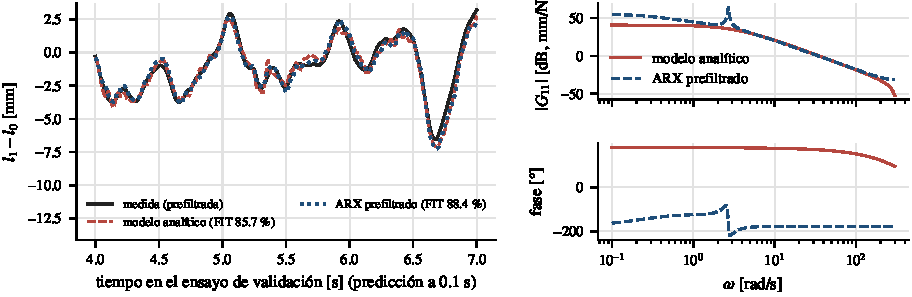
\includegraphics[width=\columnwidth]{identificacion.pdf}
\caption{Validación de la identificación: longitud medida y predicha a 0.1~s.}
\label{fig:id}
\end{figure}

% =====================================================================================================
\section{Trayectorias de referencia óptimas}\label{sec:var}

\subsection{Primera variación y condiciones de frontera}

La trayectoria que minimiza $\mathcal J[x] = \int_{t_0}^{t_f}F(t, x, \dot x)\,dt$ se obtiene perturbando $x = x^\star + \epsilon\eta$. Integrando por partes,
\begin{equation}
\delta\mathcal J = \bigl[F_{\dot x}\eta\bigr]_{t_0}^{t_f} + \int_{t_0}^{t_f}\Bigl(F_x - \frac{d}{dt}F_{\dot x}\Bigr)\eta\,dt = 0 .
\label{eq:dJ}
\end{equation}
Por el lema fundamental, en el interior se cumple la ecuación de Euler--Lagrange, $F_x - \frac{d}{dt}F_{\dot x} = 0$ \cite{gelfand1963}. En cada extremo, o el valor es conocido ($\eta = 0$), o es libre y debe cumplirse la condición natural $F_{\dot x} = 0$. Desarrollando la derivada total,
\begin{equation}
F_x - F_{\dot xt} - F_{\dot xx}\dot x - F_{\dot x\dot x}\ddot x = 0 ,
\label{eq:ELdes}
\end{equation}
que es una ecuación de segundo orden si $F_{\dot x\dot x} \ne 0$. Además, para cualquier extremal,
\begin{equation}
\frac{d}{dt}\bigl(\dot xF_{\dot x} - F\bigr) = \dot x\Bigl(\frac{d}{dt}F_{\dot x} - F_x\Bigr) - F_t = -F_t ,
\label{eq:beltrami}
\end{equation}
de modo que la dependencia de $F$ determina cuántas integraciones se ahorran. La Tabla~\ref{tab:casos} resume los cuatro casos.

\begin{table}[t]
\centering
\caption{Casos especiales del integrando}
\label{tab:casos}
\footnotesize
\setlength{\tabcolsep}{3pt}
\begin{tabularx}{\columnwidth}{@{}c>{\centering\arraybackslash}p{1.25cm}>{\raggedright\arraybackslash}X>{\raggedright\arraybackslash}p{2.1cm}@{}}
\toprule
Caso & Integrando & Simplificación & En la plataforma \\
\midrule
I & $F(t, \dot x)$ & $F_x = 0 \Rightarrow F_{\dot x} = c$ (integral primera) & Intercepción de una referencia móvil \\
II & $F(t, x, \dot x)$ & Ecuación~\eqref{eq:ELdes} completa; $F_t \ne 0$, sin integral primera & Descuento; seguimiento de una onda \\
III & $F(x, \dot x)$ & $F_t = 0$ en~\eqref{eq:beltrami} $\Rightarrow \dot xF_{\dot x} - F = C$ (Beltrami) & Extremos fijos, final libre, tiempo libre \\
IV & $F(t, x)$ & $F_{\dot x} = 0 \Rightarrow F_x(t, x) = 0$ (algebraica) & Equilibrio estático \\
\bottomrule
\end{tabularx}
\end{table}

\textbf{Condiciones de segundo orden.} Con $x = x^\star + \epsilon\eta$, la segunda variación es
\begin{equation}
\delta^2\mathcal J = \frac12\int_{t_0}^{t_f}\bigl(F_{xx}\eta^2 + 2F_{x\dot x}\eta\dot\eta + F_{\dot x\dot x}\dot\eta^2\bigr)dt .
\label{eq:d2J}
\end{equation}
Integrando por partes el término cruzado, $\int2F_{x\dot x}\eta\dot\eta\,dt = -\int\frac{d}{dt}F_{x\dot x}\,\eta^2dt$ para $\eta(t_0) = \eta(t_f) = 0$, y~\eqref{eq:d2J} queda como $\frac12\int(P\dot\eta^2 + Q\eta^2)dt$ con $P = F_{\dot x\dot x}$ y $Q = F_{xx} - \frac{d}{dt}F_{x\dot x}$. La condición necesaria de Legendre es $P \ge 0$; la condición suficiente exige además $P > 0$ y que la ecuación de Jacobi
\begin{equation}
\frac{d}{dt}\bigl(P\dot h\bigr) - Qh = 0,\qquad h(t_0) = 0,\ \dot h(t_0) = 1,
\label{eq:jacobi}
\end{equation}
no tenga ceros en $(t_0, t_f]$, es decir, que no existan puntos conjugados \cite{gelfand1963}.

\subsection{Maniobra de referencia y casos II--IV}

Para ir de $q_A$ a $q_B$ en $T = 2$~s se usa el error normalizado $\varepsilon = (q - q_B)/(q_A - q_B)$, con $\varepsilon(0) = 1$, y el funcional
\begin{equation}
\mathcal J[\varepsilon] = \int_0^T\Bigl(\tfrac12\dot\varepsilon^2 + \tfrac12a^2\varepsilon^2\Bigr)dt,\qquad a = 2\ \text{s}^{-1},
\label{eq:Fvar}
\end{equation}
que pondera la velocidad, proporcional a la de las patas, y la distancia al destino. Euler--Lagrange da $\ddot\varepsilon - a^2\varepsilon = 0$, cuya solución general es $\varepsilon = C_1\cosh at + C_2\sinh at$.

\textbf{Caso III con extremos fijos.} Imponiendo $\varepsilon(0) = 1$ y $\varepsilon(T) = 0$,
\begin{gather}
\varepsilon^\star(t) = \frac{\sinh a(T - t)}{\sinh aT}, \label{eq:fijos}\\
\mathcal J^\star = \tfrac12[\varepsilon\dot\varepsilon]_0^T = \tfrac12a\coth aT = 1.00067 ,\nonumber
\end{gather}
donde el costo se obtuvo integrando por partes $\int\dot\varepsilon^2dt$ y usando $\ddot\varepsilon = a^2\varepsilon$. La integral de Beltrami, $\frac12\dot\varepsilon^2 - \frac12a^2\varepsilon^2 = C$, vale $C = a^2/(2\sinh^2aT) = 2.69\times10^{-3}$ en todo instante porque $\cosh^2 - \sinh^2 = 1$. En~\eqref{eq:jacobi}, $P = 1$ y $Q = a^2$, de modo que $\ddot h = a^2h$ con $h(0) = 0$ y $\dot h(0) = 1$ da $h = \sinh(at)/a$, que no se anula para $t > 0$: no hay puntos conjugados para ningún $T$. La condición de Legendre, $F_{\dot\varepsilon\dot\varepsilon} = 1 > 0$, y la hessiana $\mathrm{diag}(a^2, 1) \succ 0$ muestran además que $F$ es estrictamente convexa y que el extremal es el mínimo global. Con perturbaciones de Ritz, $\eta = \sum_nb_n\sin(n\pi t/T)$, el término lineal es $\delta\mathcal J = 0$ y
\begin{equation}
\mathcal J = \mathcal J^\star + \sum_n\kappa_nb_n^2,\quad \kappa_n = \frac{T}{4}\Bigl[\Bigl(\frac{n\pi}{T}\Bigr)^2 + a^2\Bigr],
\end{equation}
con $\kappa_1 = 3.234$, $\kappa_2 = 6.935$ y $\kappa_3 = 13.10$: un paraboloide con vértice en el óptimo.

\textbf{Caso III con final libre o tiempo libre.} Si $\varepsilon(T)$ es libre, la condición natural $\dot\varepsilon(T) = 0$ da $\varepsilon^\star = \cosh a(T - t)/\cosh aT$: la plataforma llega en reposo sin imponerlo, con $\mathcal J^\star = \frac12a\tanh aT = 0.99933$ y un error residual de $1/\cosh aT = 3.7$~\%. Si $T$ es libre, la transversalidad exige $[F - \dot\varepsilon F_{\dot\varepsilon}]_T = -C = 0$, es decir, $\dot\varepsilon = -a\varepsilon$: decaimiento exponencial con constante de tiempo $1/a = 0.5$~s.

\textbf{Caso II.} Con un factor de descuento, $L = e^{-\alpha t}F$, la ecuación es $\ddot\varepsilon - \alpha\dot\varepsilon - a^2\varepsilon = 0$, con raíces $r_{1,2} = \frac12(\alpha\pm\sqrt{\alpha^2 + 4a^2}) = 2.562$ y $-1.562$~s$^{-1}$ para $\alpha = 1$~s$^{-1}$. La plataforma avanza más despacio al comienzo: $\varepsilon(1\ \text{s}) = 0.206$ frente a $0.133$ sin descuento.

\textbf{Caso IV.} Sin $\dot x$ la ecuación es algebraica; en la plataforma corresponde al equilibrio estático $\vect J_0\T\vect F_0 = \vect g_0$.

\textbf{Caso multivariable.} Con $\vect e = \vect q - \vect q_B$ y $F = \frac12\dot{\vect e}\T\vect M_0\dot{\vect e} + \frac12\vect e\T\vect K\vect e$, $\vect K = a^2\mathrm{diag}(\vect M_0)$, Euler--Lagrange da $\ddot{\vect e} = \vect M_0^{-1}\vect K\vect e$. Descomponiendo en modos, cada uno sigue~\eqref{eq:fijos} con su frecuencia, $\omega_k = \{\omegaMulti\}$~s$^{-1}$. Como $\vect M_0$ es casi diagonal, las seis frecuencias difieren de $a$ en el cuarto decimal y el caso escalar basta.

\subsection{Caso I: intercepción de una referencia móvil}

Desde $z_0 = 5$~mm en reposo se intercepta $\phi(t) = A\sin\omega t$ ($A = 15$~mm, $\omega = 2.827$~rad/s) con $F = \frac12\dot z^2$ y $T$ libre. Como $F_z = 0$, $\dot z = c$ y la trayectoria es una recta. La primera variación con extremo móvil da $\delta\mathcal J = F_{\dot z}\delta z_T + (F - \dot zF_{\dot z})\delta T$; con el punto final sobre la curva, $\delta z_T = \dot\phi(T)\delta T$, y la transversalidad queda
\begin{equation}
\Bigl[F + F_{\dot z}(\dot\phi - \dot z)\Bigr]_T = c\Bigl(\dot\phi(T) - \tfrac{c}{2}\Bigr) = 0\ \Rightarrow\ c = 2\dot\phi(T).
\end{equation}
La condición de encuentro $z_0 + 2A\omega\cos(\omega T)\,T = A\sin\omega T$ se resuelve por Newton en tres iteraciones: $T = 0.470$~s y $c = 20.35$~mm/s.

\subsection{Casos de frontera A--D}

Combinando inicio y final conocidos o libres se obtienen cuatro casos: A (ambos conocidos), B (final libre), C (inicio libre) y D (ambos libres). Como liberar un extremo agranda el conjunto admisible, $\mathcal J^\star_D \le \mathcal J^\star_B, \mathcal J^\star_C \le \mathcal J^\star_A$. Con una referencia fija los casos de inicio libre son triviales; por eso se aplicaron al seguimiento de media onda en $z$, $r = A\cos\omega t$ ($A = \AOnda$~mm, \fOnda{}~Hz, $T = \TOnda$~s), con
\begin{equation}
F = \tfrac12\dot x^2 + \tfrac12a^2\bigl(x - r(t)\bigr)^2\ \Rightarrow\ \ddot x - a^2x = -a^2r(t),
\end{equation}
que es el caso II. La solución particular $x_p = \kappa r$ cumple $-\omega^2\kappa - a^2\kappa = -a^2$, es decir, $\kappa = a^2/(a^2 + \omega^2) = \kappaOnda$, y la general es
\begin{equation}
x(t) = \kappa r(t) + C_1e^{-at} + C_2e^{-a(T - t)} .
\label{eq:xonda}
\end{equation}
Cada caso impone dos ecuaciones lineales en $(C_1, C_2)$: $x = 0$ en un extremo conocido y $\dot x = 0$ en uno libre. En el caso A, por Cramer, $C_{1,2} = \mp10.83$~mm; en D, como $\dot r(0) = \dot r(T) = 0$, el sistema es homogéneo y $x^\star = \kappa r$. La Tabla~\ref{tab:frontera} y la Fig.~\ref{fig:frontera} confirman el orden de los costos.

\begin{table}[t]
\centering
\caption{Casos de frontera: extremos de la trayectoria [mm] y costo [mm$^2$/s]}
\label{tab:frontera}
\footnotesize
\setlength{\tabcolsep}{2.5pt}
\begin{tabular}{@{}clllrrr@{}}
\toprule
Caso & Inicio & Final & Condiciones & $z^\star(0)$ & $z^\star(T)$ & $\mathcal J^\star$ \\
\midrule
\tabinput{../desarrollo_matematico/tablas/frontera.tex}
\bottomrule
\end{tabular}
\end{table}

\begin{figure}[t]
\centering
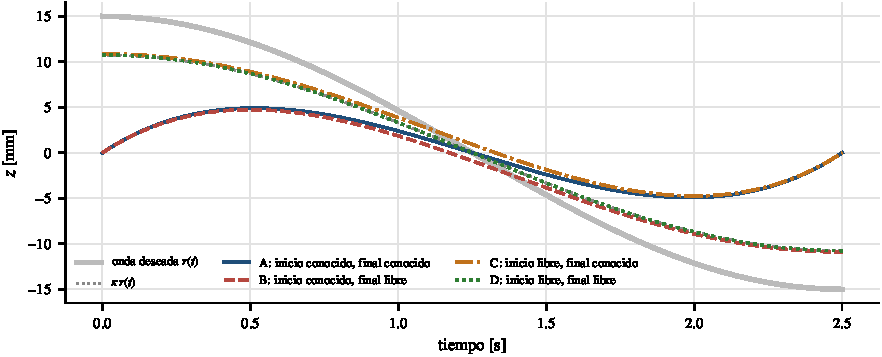
\includegraphics[width=\columnwidth]{casos_frontera.pdf}
\caption{Casos de frontera A--D aplicados a la onda en $z$: los extremos conocidos llegan a cero y los libres, con pendiente nula.}
\label{fig:frontera}
\end{figure}

\subsection{Principio del mínimo de Pontryagin}

Para $\dot{\vect x} = \vect f(\vect x, \vect u)$ y $\mathcal J = \int L\,dt$, se adjunta la dinámica con el coestado $\boldsymbol\lambda$ y se define $\mathcal H = L + \boldsymbol\lambda\T\vect f$. Anulando la primera variación del funcional aumentado se obtienen \cite{kirk1970}
\begin{equation}
\dot{\vect x} = \frac{\partial\mathcal H}{\partial\boldsymbol\lambda},\qquad \dot{\boldsymbol\lambda} = -\frac{\partial\mathcal H}{\partial\vect x},\qquad \vect u^\star = \arg\min_{\vect u\in\mathcal U}\mathcal H .
\end{equation}
Con $\dot\varepsilon = u$ y $L = \frac12u^2 + \frac12a^2\varepsilon^2$, $u^\star = -\lambda$ y $\dot\lambda = -a^2\varepsilon$ reproducen $\ddot\varepsilon = a^2\varepsilon$; $\mathcal H^\star = -C$ es la integral de Beltrami, el final libre corresponde a $\lambda(T) = 0$ y el tiempo libre a $\mathcal H(T) = 0$.

\textbf{Mínima energía.} Para una pata como doble integrador, $m\ddot l = u$ con $m = \mEff$~kg y $\mathcal J = \int u^2dt$, $\mathcal H = u^2 + \lambda_1v + \lambda_2u/m$. Entonces $\dot\lambda_1 = 0$, $\lambda_2$ es lineal en $t$ y $u^\star = -\lambda_2/2m$ también. Imponiendo reposo en $l = 0$ y en $l = \Delta l$,
\begin{gather}
u^\star = \frac{6m\Delta l}{T^2}\Bigl(1 - \frac{2t}{T}\Bigr),\nonumber\\ l = \Delta l(3\tau^2 - 2\tau^3),\qquad E^\star = \frac{12m^2\Delta l^2}{T^3},
\end{gather}
con $\tau = t/T$. Para $\Delta l = 14.26$~mm en 2~s, $u^\star(0) = \uEnMax$~mN.

\textbf{Tiempo mínimo.} Con $|\ddot l| \le \ddot l_{\max} = \aMax$~m/s$^2$ y $L = 1$, $\mathcal H = 1 + \lambda_1v + \lambda_2\ddot l$ es lineal en el control, que toma su valor extremo: $\ddot l^\star = -\ddot l_{\max}\mathrm{sign}\,\lambda_2$ (bang-bang). Como $\lambda_2$ es una recta, hay a lo sumo una conmutación, que por simetría ocurre en $T/2$:
\begin{equation}
T = 2\sqrt{\Delta l/\ddot l_{\max}} = 2\sqrt{0.02319/0.08} = \TMin\ \text{s}
\end{equation}
para la pata más exigida, con velocidad pico de \vPico~mm/s. Con $e = l - \Delta l$, en cada arco $\ddot e = \mp\ddot l_{\max}$ es constante y $v\,dv = \mp\ddot l_{\max}\,de$, de modo que las trayectorias son parábolas; la única que llega al origen frenando define la curva de conmutación
\begin{equation}
e = -\frac{v\lvert v\rvert}{2\ddot l_{\max}},
\end{equation}
y la ley en lazo cerrado es $\ddot l^\star = -\ddot l_{\max}\,\mathrm{sign}\bigl(e + v\lvert v\rvert/2\ddot l_{\max}\bigr)$. El coestado confirma el número de conmutaciones: $\dot\lambda_1 = -\partial\mathcal H/\partial l = 0$ y $\dot\lambda_2 = -\partial\mathcal H/\partial v = -\lambda_1$ dan $\lambda_2 = c_2 - c_1t$, que cambia de signo a lo sumo una vez. Las demás patas recorren su elongación en la misma proporción, de modo que la plataforma se mueve en línea recta entre las dos configuraciones.

\begin{figure*}[t]
\centering
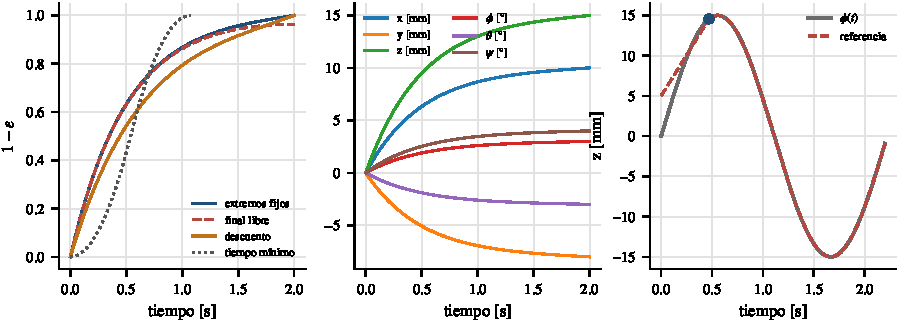
\includegraphics[width=\textwidth]{trayectorias_variacionales.pdf}
\caption{Trayectorias variacionales: fracción recorrida $1 - \varepsilon(t)$ en los casos escalares y en tiempo mínimo (izquierda), componentes de la maniobra de 6~GDL (centro) e intercepción de la senoidal (derecha).}
\label{fig:trayvar}
\end{figure*}

% =====================================================================================================
\section{Control PID descentralizado}\label{sec:pid}

\subsection{Modelo de una pata y discretización}

Cada pata se controla con un PID sobre su error de longitud, con la referencia obtenida por~\eqref{eq:ik}. El término diagonal de~\eqref{eq:patas} da $m\,\delta\ddot l = \delta F + k\,\delta l$, con $m = \mLeg$~kg y $k = \kLeg$~N/m:
\begin{equation}
G(s) = \frac{1/m}{(s - \sigma)(s + \sigma)},\quad \sigma = \sqrt{k/m} = \sigmaLeg\ \text{s}^{-1}.
\end{equation}
Con retenedor de orden cero, $G(z) = (1 - z^{-1})\mathcal Z\{G(s)/s\}$. Las fracciones parciales $\frac{1}{s(ms^2 - k)} = \frac1k\bigl[-\frac1s + \frac{1/2}{s - \sigma} + \frac{1/2}{s + \sigma}\bigr]$ y $\mathcal Z\{1/(s\mp\sigma)\} = z/(z - e^{\pm\sigma T_s})$ dan
\begin{equation}
G(z) = \frac{c - 1}{k}\cdot\frac{z + 1}{z^2 - 2cz + 1},\quad c = \cosh\sigma T_s ,
\label{eq:Gz}
\end{equation}
con $c = \cLeg$ y polos en $\zUnst$ y $\zSt$.

\subsection{Ley de control}

La fuerza de cada pata es la de equilibrio más las tres acciones,
\begin{equation}
F_i(k) = F_0 + K_pe_i(k) + K_ix_{I,i}(k) + K_dd_i(k),
\end{equation}
con $e_i = l_{i,r} - l_i$,
con integrador rectangular $x_{I,i}(k+1) = x_{I,i}(k) + T_se_i(k)$ y derivada filtrada. El filtro $K_ds/(1 + s/\omega_f)$, con $\omega_f = 160$~rad/s, discretizado de forma exacta suponiendo constante la diferencia de error en cada periodo, da
\begin{equation}
d_i(k) = \alpha\,d_i(k-1) + (1 - \alpha)\frac{e_i(k) - e_i(k-1)}{T_s},
\end{equation}
con $\alpha = e^{-\omega_fT_s} = \alphaD$.
Un anti-\textit{windup} condicional congela el integrador cuando la fuerza satura y el error la empuja hacia el límite. Transformando cada ecuación y llevando todo al denominador común $(z - 1)(z - \alpha)$,
\begin{equation}
C(z) = \frac{n_2z^2 + n_1z + n_0}{(z - 1)(z - \alpha)},
\end{equation}
\begin{equation*}
\begin{aligned}
n_2 &= K_p + D,\qquad n_0 = \alpha K_p - \alpha K_iT_s + D,\\
n_1 &= -(1 + \alpha)K_p + K_iT_s - 2D,
\end{aligned}
\end{equation*}
con $D = K_d(1 - \alpha)/T_s$.

\subsection{Condición de estabilidad}

En tiempo continuo y sin filtro, $1 + C(s)G(s) = 0$ con $C = K_p + K_i/s + K_ds$ da el polinomio característico
\begin{equation}
ms^3 + K_ds^2 + (K_p - k)s + K_i = 0 .
\end{equation}
El arreglo de Routh es
\begin{equation}
\begin{array}{c|cc}
s^3 & m & K_p - k\\
s^2 & K_d & K_i\\
s^1 & b_1 & 0\\
s^0 & K_i &
\end{array}\qquad b_1 = \frac{K_d(K_p - k) - mK_i}{K_d},
\end{equation}
y su primera columna $\{m,\ K_d,\ b_1,\ K_i\}$ no presenta cambios de signo si y solo si
\begin{equation}
K_d > 0,\qquad K_i > 0,\qquad K_p > k + \frac{mK_i}{K_d} .
\label{eq:routh}
\end{equation}
Sin derivativa falta el término en $s^2$ y no existe ninguna ganancia estabilizante; la proporcional debe superar la rigidez negativa, y en el lazo MIMO la cota~\eqref{eq:cotaKp}.

\subsection{Ganancias y propiedades del lazo}

Las ganancias se obtienen como factores de escala sobre un diseño base, $K = sK^0$ con $K^0 = (\KpBase, \KiBase, \KdBase)$, ajustados en la sección~\ref{sec:opt}:
\begin{equation}
K_p = \KpOpt\ \tfrac{\text{N}}{\text{m}},\quad K_i = \KiOpt\ \tfrac{\text{N}}{\text{m\,s}},\quad K_d = \KdOpt\ \tfrac{\text{N\,s}}{\text{m}},
\end{equation}
es decir, $T_i = K_p/K_i = \TiOpt$~s y $T_d = K_d/K_p = \TdOpt$~ms. La condición~\eqref{eq:routh} se cumple con holgura: $K_d(K_p - k) = 460\,870 > mK_i = 80\,436$, y $k + mK_i/K_d = 948.2 < 4556.7$~N/m. Las raíces continuas son $\RootsCont$~s$^{-1}$.

\textbf{Lazo discreto de una pata.} Con~\eqref{eq:Gz} y $C(z)$, la ecuación característica $1 + C(z)G(z) = 0$ multiplicada por $k(z - 1)(z - \alpha)(z^2 - 2cz + 1)$ es
\begin{equation}
\begin{split}
k(z - 1)(z - \alpha)(z^2 - 2cz + 1)&\\ + (c - 1)(z + 1)(n_2z^2 + n_1z + n_0) &= 0 ,
\end{split}
\end{equation}
un polinomio de cuarto grado, $\charPoly = 0$, con raíces $\charRoots$ dentro del círculo unitario: radio espectral $\rhoSiso < 1$. El polo más lento, $z = \rhoSiso$, corresponde a $s = \ln(\rhoSiso)/T_s = -4.7$~s$^{-1}$ y lo fija la acción integral.

\textbf{Error en régimen permanente.} La ganancia de lazo $L(s) = C(s)G(s) = (K_ds^2 + K_ps + K_i)/[s(ms^2 - k)]$ tiene un polo en el origen, de modo que el lazo es de tipo~1. Por el teorema del valor final, ante un escalón $R/s$ el error es $e_{ss} = \lim_{s\to0}sR/[s(1 + L)] = 0$; ante una rampa $v/s^2$,
\begin{equation}
e_{ss} = \frac{v}{\lim_{s\to0}sL(s)} = \frac{v}{K_i/(-k)} = -\frac{k}{K_i}v ,
\end{equation}
es decir, $|e_{ss}| = (\kLeg/\KiOpt)\,v \approx 0.010\,v$ (10~ms por unidad de velocidad de la pata), con signo opuesto al usual porque la rigidez de la planta es negativa.

La Fig.~\ref{fig:lcl} (derecha) muestra el escalón de una pata con el PID óptimo sobre el modelo discreto: el sobrepico es del 48~\% y el tiempo de establecimiento al 2~\%, de 0.50~s. Los ceros de $C(s)$, raíces de $K_ds^2 + K_ps + K_i$, están en $-4.52$ y $-38.7$~s$^{-1}$: el primero casi cancela el polo real $-4.64$, y el sobrepico lo fijan el par complejo $-9.77 \pm 28.57j$, con $\zeta = 9.77/\sqrt{9.77^2 + 28.57^2} = 0.32$, y el cero en $-38.7$, que adelanta la respuesta.

Con $s = j\omega$, $|G| = 1/(m\omega^2 + k)$ y $\angle G = -180^\circ$ más el retardo de medio periodo del retenedor. Separando el término derivativo en parte real e imaginaria, $\mathrm{Re}\,C = K_p + K_d\omega^2/\omega_f/(1 + \omega^2/\omega_f^2)$ y $\mathrm{Im}\,C = -K_i/\omega + K_d\omega/(1 + \omega^2/\omega_f^2)$. En $\omega = \wcHand$~rad/s, $|C| = \CwcMag$~N/m y $|G| = \GwcMag$~m/N, cuyo producto es $0.999$: ese es el cruce, con $\angle C = \CwcAng^\circ$ y un margen de fase estimado de \PMhand$^\circ$, aportado íntegramente por la acción derivativa. El cálculo exacto sobre el lazo MIMO discreto, abriendo la pata 1 con las demás controladas,
\begin{equation}
L_1(z) = C(z)\bigl[G_{11} - \vect G_{1r}C(\vect I + \vect G_{rr}C)^{-1}\vect G_{r1}\bigr],
\end{equation}
da $\omega_c = \wcPid$~rad/s, margen de fase de \PMPid$^\circ$, margen de ganancia de \GMPid~dB y pico de sensibilidad $M_s = \MsPid$ (Fig.~\ref{fig:pidfrec}). La diferencia con el cálculo a mano se debe a que este usa la masa de la pata con las demás quietas, \mLeg~kg, mientras que con las patas controladas la masa efectiva es \mEff~kg. El lazo MIMO completo tiene 30 estados (12 de la planta y 6 por cada integrador, error anterior y derivada filtrada) y radio espectral \rhoPid.

\begin{figure}[t]
\centering
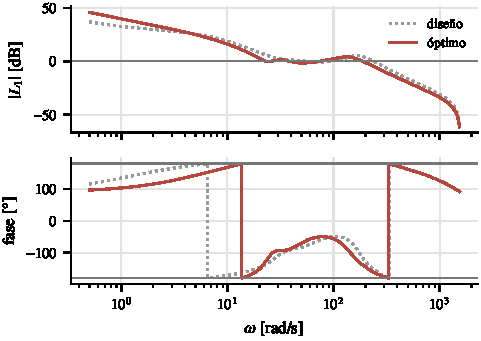
\includegraphics[width=\columnwidth]{pid_frecuencia.pdf}
\caption{Respuesta en frecuencia del lazo abierto de la pata 1 con el PID óptimo.}
\label{fig:pidfrec}
\end{figure}

% =====================================================================================================
\section{Realimentación de estados con observador de Luenberger}\label{sec:ss}

\subsection{Sistema aumentado y asignación de estructura propia}

Para anular el error estacionario se agrega un integrador por coordenada, $\dot{\vect z} = \delta\vect r - \vect C_y\delta\vect x$, y el sistema aumentado de 18 estados es
\begin{equation}
\begin{bmatrix}\delta\dot{\vect x}\\ \dot{\vect z}\end{bmatrix} = \underbrace{\begin{bmatrix}\vect A & \vect 0\\ -\vect C_y & \vect 0\end{bmatrix}}_{\vect A_a}\begin{bmatrix}\delta\vect x\\ \vect z\end{bmatrix} + \underbrace{\begin{bmatrix}\vect B\\ \vect 0\end{bmatrix}}_{\vect B_a}\delta\vect u + \begin{bmatrix}\vect 0\\ \vect I\end{bmatrix}\delta\vect r ,
\end{equation}
controlable porque $(\vect A, \vect B)$ lo es y no hay ceros en el origen. La ley es $\delta\vect u = -\vect K\hat{\vect x} + \vect K_i\vect z + \vect N_r\delta\vect r = -\vect K_a\vect x_a + \vect N_r\delta\vect r$, con $\vect K_a = [\vect K\;\;-\vect K_i]$. La ganancia se obtiene asignando a cada polo $\lambda_j$ una dirección de entrada $\vect g_j\in\mathbb R^6$ \cite{moore1976}:
\begin{equation}
\vect v_j = (\vect A_a - \lambda_j\vect I)^{-1}\vect B_a\vect g_j,\qquad \vect K_a\vect v_j = \vect g_j .
\end{equation}
Entonces $(\vect A_a - \vect B_a\vect K_a)\vect v_j = \lambda_j\vect v_j + \vect B_a\vect g_j - \vect B_a\vect g_j = \lambda_j\vect v_j$, y con $\vect V = [\vect v_1\cdots\vect v_{18}]$ y $\vect G = [\vect g_1\cdots\vect g_{18}]$,
\begin{equation}
\vect K_a = \vect G\vect V^{-1}.
\end{equation}
La construcción exige que $\lambda_j\notin\lambda(\vect A_a)$, para que $\vect A_a - \lambda_j\vect I$ sea invertible, y que $\vect V$ tenga rango completo. Por el teorema de Moore \cite{moore1976}, un conjunto de vectores propios $\{\vect v_j\}$ es asignable si y solo si los $\vect v_j$ son linealmente independientes, $\vect v_j = \bar{\vect v}_k$ cuando $\lambda_j = \bar\lambda_k$, y cada $\vect v_j$ pertenece al subespacio $\mathrm{Im}\,(\vect A_a - \lambda_j\vect I)^{-1}\vect B_a$, de dimensión $\mathrm{rango}\,\vect B_a = 6$. Con seis entradas, además de fijar cada valor propio se puede elegir su vector propio dentro de un subespacio de dimensión seis; la elección de $\vect g_j$ usa esa libertad para desacoplar los ejes.
Las direcciones $\vect g_j$ son columnas normalizadas de $\vect B_2^{-1}$, de modo que cada par de polos actúa sobre un eje cartesiano; los pares conjugados comparten $\vect g_j$ y $\vect K_a$ resulta real. Los polos de diseño, de $-25.5 \pm 9j$ a $-30 \pm 12j$ ($\zeta = 0.93$--$0.94$) y los integradores de $-4.5$ a $-6$~s$^{-1}$, se escalan por un factor $\alpha$; con el óptimo, $\alpha = \alphaOpt$, el par oscilatorio más lento es $\PoloCtrl$, con constante de tiempo $1/85.6 = 11.7$~ms, y los seis polos de los integradores quedan en $-4.5\alpha$ a $-6\alpha$, es decir, entre $-15.1$ y $-20.1$~s$^{-1}$; estos últimos son los dominantes y fijan el establecimiento, del orden de $4/\lvert\lambda\rvert = 0.20$--$0.26$~s.

En el modelo lineal discreto con el estimador actual, los escalones en $x$, $z$ y $\psi$ se establecen al 2~\% en 0.20~s con sobrepicos del 16 al 17~\%, y la salida en los demás ejes no supera el 1.4~\% de la referencia (Fig.~\ref{fig:lcl}, izquierda): la misma respuesta normalizada en las tres direcciones es consecuencia de asignar los mismos polos a cada eje cartesiano a través de $\vect g_j$.

\begin{figure*}[t]
\centering
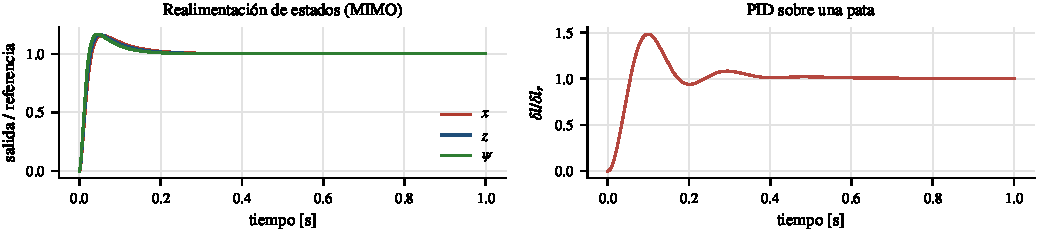
\includegraphics[width=\textwidth]{lazo_cerrado_lineal.pdf}
\caption{Escalones en el modelo lineal discreto: realimentación de estados con estimador actual (izquierda, salidas normalizadas) y PID sobre una pata (derecha).}
\label{fig:lcl}
\end{figure*}

\subsection{Precompensador}

Sin integrador, en régimen estacionario $\vect 0 = (\vect A - \vect B\vect K)\delta\vect x_{ss} + \vect B\vect N_r\delta\vect r$; pidiendo $\vect C_y\delta\vect x_{ss} = \delta\vect r$ para todo $\delta\vect r$,
\begin{equation}
\vect N_r = -\bigl[\vect C_y(\vect A - \vect B\vect K)^{-1}\vect B\bigr]^{-1} = \vect K_{pos} - \vect B_2^{-1}\vect A_{21},
\end{equation}
donde la segunda forma se obtiene por bloques con $\vect K = [\vect K_{pos}\;\vect K_{vel}]$. En régimen estacionario la fila de posición de~\eqref{eq:AB} da $\delta\dot{\vect q}_{ss} = \vect 0$, y la de velocidad,
\begin{equation}
\vect 0 = \vect A_{21}\delta\vect q_{ss} + \vect B_2\bigl(-\vect K_{pos}\delta\vect q_{ss} + \vect N_r\delta\vect r\bigr);
\end{equation}
imponiendo $\delta\vect q_{ss} = \delta\vect r$ y multiplicando por $\vect B_2^{-1}$ resulta la expresión anterior. Así, $\vect K_{pos}$ restituye la acción proporcional y $-\vect B_2^{-1}\vect A_{21} = \vect J_0^{-\top}\vect K_q$ entrega la fuerza que sostiene la nueva configuración contra la rigidez negativa. El integrador discreto, saturado en $|z_j| \le 0.05$~m\,s, tiene como punto fijo $\delta\vect y = \delta\vect r$, de modo que el error estacionario es nulo aunque $\vect N_r$ no sea exacto.

\subsection{Observador de Luenberger}

Solo se miden las posiciones; derivarlas amplifica el ruido, por lo que las velocidades se estiman con un observador de Luenberger \cite{luenberger1971}. En tiempo continuo, $\dot{\hat{\vect x}} = \vect A\hat{\vect x} + \vect B\vect u + \vect L(\vect y - \vect C_y\hat{\vect x})$ y el error $\vect e = \vect x - \hat{\vect x}$ cumple $\dot{\vect e} = (\vect A - \vect L\vect C_y)\vect e$, independiente de $\vect u$. Como $\lambda(\vect A - \vect L\vect C_y) = \lambda(\vect A\T - \vect C_y\T\vect L\T)$, la ganancia se calcula por dualidad con el mismo método de asignación.

Se implementa como estimador actual \cite{franklin1998}, que usa la medida $\vect y(k)$ antes de calcular $\vect u(k)$:
\begin{align}
\hat{\vect x}_c(k) &= \hat{\vect x}_p(k) + \vect L_d\bigl(\delta\vect y(k) - \vect C_d\hat{\vect x}_p(k)\bigr),\\
\hat{\vect x}_p(k+1) &= \vect A_d\hat{\vect x}_c(k) + \vect B_d\delta\vect u(k).
\end{align}
Restando estas ecuaciones de las de la planta,
\begin{gather}
\vect e_p(k+1) = \vect A_d(\vect I - \vect L_d\vect C_d)\vect e_p(k),\nonumber\\ \vect e_c(k+1) = (\vect A_d - \vect L_d\vect C_d\vect A_d)\vect e_c(k),
\end{gather}
que tienen los mismos polos porque $\lambda(\vect X\vect Y) = \lambda(\vect Y\vect X)$; $\vect L_d$ se calcula por dualidad con $(\vect A_d\T, (\vect C_d\vect A_d)\T)$. Los polos de diseño, de $-78 \pm 18j$ a $-100.5 \pm 25.5j$, se escalan por $\beta$ y se llevan a $z = e^{\beta\mu T_s}$. Con el óptimo, $\beta = \betaOpt$, el polo dominante es $\PoloObs$~s$^{-1}$ ($|z| = \obsZmax$): el observador resulta tres veces más lento que el par oscilatorio del controlador ($-27.5$ frente a $-85.6$~s$^{-1}$), aunque más rápido que los integradores.
La Fig.~\ref{fig:obs} muestra la norma del error de velocidad del estimador partiendo de 10~mm/s y $1^\circ$/s: decae como $\rho^k$ con $\rho = \obsZmax$, el radio espectral de $\vect A_o$.

\begin{figure}[t]
\centering
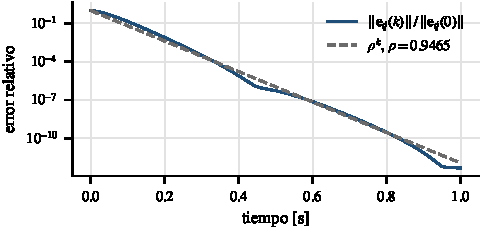
\includegraphics[width=\columnwidth]{observador_error.pdf}
\caption{Convergencia del error de velocidad del estimador actual frente a la cota $\rho^k$.}
\label{fig:obs}
\end{figure}

\textbf{Propagación del ruido.} Con la medida $\delta\vect y(k) = \vect C_d\vect x(k) + \vect v(k)$ y ruido blanco de covarianza $\sigma^2\vect I$, el error del estimador actual cumple $\vect e_c(k+1) = \vect A_o\vect e_c(k) - \vect L_d\vect v(k+1)$ con $\vect A_o = \vect A_d - \vect L_d\vect C_d\vect A_d$. Su covarianza estacionaria $\vect P = \mathrm{E}[\vect e_c\vect e_c\T]$ es la solución de la ecuación discreta de Lyapunov
\begin{equation}
\vect P = \vect A_o\vect P\vect A_o\T + \sigma^2\vect L_d\vect L_d\T ,
\label{eq:lyapobs}
\end{equation}
que existe y es única porque $\vect A_o$ es estable. Un observador más rápido tiene $\vect L_d$ mayor y, por~\eqref{eq:lyapobs}, más varianza de estimación, que la ganancia $\vect K$ convierte en fuerza: el compromiso entre velocidad y ruido es el que resuelve el criterio de la sección~\ref{sec:opt}.

\subsection{Principio de separación}

Con $\hat{\vect x}_c = \vect x - (\vect I - \vect L_d\vect C_d)\vect e_p$ y $\delta\vect r = \vect 0$, el lazo cerrado discreto con integradores es
\begin{equation}
{\setlength{\arraycolsep}{2pt}\small
\begin{bmatrix}\vect x\\ \vect z\\ \vect e_p\end{bmatrix}_{k+1} =
\begin{bmatrix}
\vect A_d - \vect B_d\vect K & \vect B_d\vect K_i & \vect B_d\vect K(\vect I - \vect L_d\vect C_d)\\
-T_s\vect C_d & \vect I & \vect 0\\
\vect 0 & \vect 0 & \vect A_d(\vect I - \vect L_d\vect C_d)
\end{bmatrix}
\begin{bmatrix}\vect x\\ \vect z\\ \vect e_p\end{bmatrix}_{k}}.
\end{equation}
Por ser triangular por bloques, su polinomio característico es el producto del de los 18 estados del controlador por el de los 12 del observador: ambos se diseñan por separado. El radio espectral del lazo es \rhoSS.

% =====================================================================================================
\section{Selección óptima de parámetros}\label{sec:opt}

Ambas estrategias se ajustan con el mismo criterio,
\begin{equation}
J = \sum_{s=1}^{5}\Bigl(\frac{\mathrm{ITAE}_s}{\mathrm{ITAE}_s^0} + 0.25\,\frac{J_{u,s}}{J_{u,s}^0}\Bigr),
\label{eq:J}
\end{equation}
\begin{equation}
\mathrm{ITAE} = \int_0^Tt\lVert\vect e(t)\rVert_1dt,\qquad J_u = \int_0^T\vect F\T\vect F\,dt ,
\end{equation}
evaluado sobre la planta no lineal~\eqref{eq:dyn} con saturación y ruido de 0.1~mm en cinco escenarios: (1) ensayo normalizado, escalón de 8~mm en $x$ y 15~mm en $z$ con un impulso de 20~N en 0.45~s; (2) carga sostenida de 0.5~kg con fuerzas externas de $-10$~N en $z$ y 4~N en $x$; (3) senoidal en $z$; (4) maniobra de 6~GDL; (5) trayectoria circular. Cada término se normaliza con el diseño inicial, de modo que $J^0 = 5\cdot1.25 = 6.25$ y el peso 0.25 da al error cuatro veces la importancia del esfuerzo. Las variables de decisión son $(\ln s_p, \ln s_i, \ln s_d)$ para el PID y $(\ln\alpha, \ln\beta)$ para la realimentación de estados; la escala logarítmica mantiene positivas las ganancias. La búsqueda combina Nelder--Mead \cite{nelder1965} desde varios puntos iniciales con una búsqueda de patrón de paso decreciente (20, 10, 5 y 2~\%). La verificación final varía cada parámetro $\pm10$~\%: en todos los casos $J$ aumenta (Tabla~\ref{tab:verif}), lo que confirma un mínimo local.

El PID óptimo alcanza $J = \JpidOpt$ y la realimentación de estados $J = \JssOpt$ (Tabla~\ref{tab:calc}). El PID mejora su diseño inicial reduciendo ambos términos; la realimentación de estados reduce el error a un tercio en las maniobras acopladas a cambio de más esfuerzo que su diseño inicial, que era muy conservador.

\begin{table}[t]
\centering
\caption{Verificación de mínimo local: $J$ al variar cada parámetro $\pm10$~\%}
\label{tab:verif}
\footnotesize
\begin{tabular}{@{}lrlrr@{}}
\toprule
Estrategia & $J^\star$ & Parámetro & $\times0.9$ & $\times1.1$ \\
\midrule
\tabinput{tablas/verificacion.tex}
\bottomrule
\end{tabular}
\end{table}

\begin{table*}[t]
\centering
\caption{Cálculo del criterio~\eqref{eq:J} en los óptimos: valores iniciales ($^0$), óptimos ($^\star$) y término de cada escenario}
\label{tab:calc}
\footnotesize
\setlength{\tabcolsep}{4pt}
\begin{tabular}{@{}lrrrrrrr@{\hspace{14pt}}rrrrrrr@{}}
\toprule
 & \multicolumn{7}{c}{PID descentralizado} & \multicolumn{7}{c}{Realimentación de estados} \\
\cmidrule(lr){2-8}\cmidrule(lr){9-15}
Escenario & ITAE$^0$ & ITAE$^\star$ & $J_u^0$ & $J_u^\star$ & $\frac{\mathrm{ITAE}^\star}{\mathrm{ITAE}^0}$ & $\frac{J_u^\star}{J_u^0}$ & Término & ITAE$^0$ & ITAE$^\star$ & $J_u^0$ & $J_u^\star$ & $\frac{\mathrm{ITAE}^\star}{\mathrm{ITAE}^0}$ & $\frac{J_u^\star}{J_u^0}$ & Término \\
\midrule
Ensayo normalizado & 0.0510 & 0.0484 & 2812.3 & 1906.6 & 0.948 & 0.678 & 1.117 & 0.1402 & 0.0473 & 942.5 & 1141.2 & 0.337 & 1.211 & 0.640 \\
Carga sostenida & 0.0504 & 0.0376 & 4270.9 & 3325.1 & 0.746 & 0.779 & 0.941 & 0.0243 & 0.0190 & 2364.5 & 2570.8 & 0.783 & 1.087 & 1.055 \\
Senoidal en $z$ & 0.0422 & 0.0332 & 2341.7 & 1411.7 & 0.786 & 0.603 & 0.936 & 0.0292 & 0.0177 & 832.9 & 853.1 & 0.606 & 1.024 & 0.862 \\
Maniobra 6 GDL & 0.0949 & 0.0645 & 2817.2 & 1820.4 & 0.680 & 0.646 & 0.841 & 0.1477 & 0.0249 & 954.3 & 1355.0 & 0.168 & 1.420 & 0.523 \\
Circular & 0.0769 & 0.0596 & 2841.6 & 1881.6 & 0.775 & 0.662 & 0.941 & 0.1232 & 0.0234 & 999.7 & 1453.0 & 0.190 & 1.453 & 0.553 \\
\midrule
$J$ (diseño: 6.25) & \multicolumn{6}{c}{} & \textbf{\JpidOpt} & \multicolumn{6}{c}{} & \textbf{\JssOpt} \\
\bottomrule
\end{tabular}
\end{table*}

% =====================================================================================================
\section{Resultados}\label{sec:resultados}

\subsection{Gemelo digital y protocolo}

Las pruebas se hicieron en un gemelo digital que integra la planta no lineal~\eqref{eq:fnl} con Runge--Kutta de cuarto orden, saturación de fuerza en $\pm\Fmax$~N, topes de carrera y ruido de medición de 0.1~mm, mientras los controladores, ambos lineales, se ejecutan cada \Ts~ms. La Tabla~\ref{tab:tabla1} reporta el ensayo normalizado del protocolo; la robustez es el aumento del RMS ante una variación de $\pm20$~\% en la ganancia de entrada $\vect B_d$, y el tiempo de cómputo es el de un paso del controlador.

\begin{table*}[t]
\centering
\caption{Comparación de estrategias (Tabla 1 del protocolo): ensayo normalizado con ruido de 0.1 mm}
\label{tab:tabla1}
\footnotesize
\setlength{\tabcolsep}{4pt}
\begin{tabular}{@{}lccc>{\raggedright\arraybackslash}p{5.8cm}cc@{}}
\toprule
Método & RMS [mm / $^\circ$] & ITAE & $J_u$ [N$^2$s] & Restricciones & Robustez & CPU [$\mu$s] \\
\midrule
\tabinput{tablas/tabla1.tex}
\midrule
MPC, LMI, robusto & \multicolumn{6}{l}{\textit{Segunda entrega}} \\
\bottomrule
\end{tabular}
\end{table*}

Las dos estrategias tienen errores parecidos en el ensayo normalizado (Fig.~\ref{fig:ensayo}). El PID rechaza mejor el impulso de 20~N, con menos de 1~mm de desviación, porque actúa sobre la medida directa de cada pata con una ganancia proporcional alta; la realimentación de estados usa un 40~\% menos de esfuerzo ($J_u = 1141$ frente a 1907~N$^2$s) y es menos sensible a la variación de los actuadores (23.0 frente a 29.5~\%), porque su precompensador entrega con el modelo la mayor parte de la fuerza necesaria.

\begin{figure}[t]
\centering
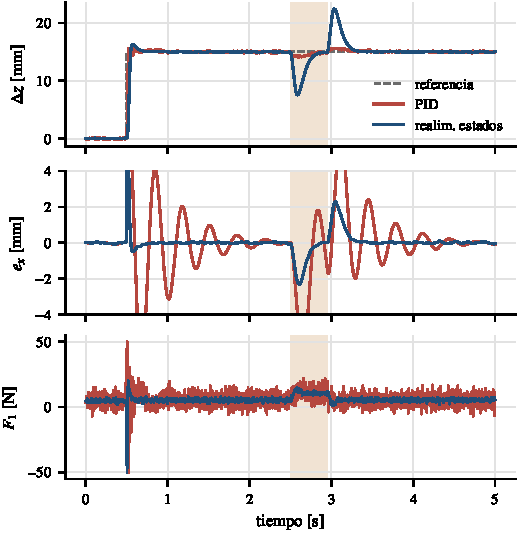
\includegraphics[width=\columnwidth]{ensayo_normalizado.pdf}
\caption{Ensayo normalizado con las ganancias óptimas: altura, error en $x$ y fuerza de la pata 1. La franja marca el impulso de 20 N.}
\label{fig:ensayo}
\end{figure}

\subsection{Cálculo previo de las referencias}

Antes de simular, cada referencia se evaluó con el modelo lineal: longitudes $\delta\vect l = \vect J_0\delta\vect q_r$, saltos en una muestra y fuerza de prealimentación
\begin{equation}
\delta\vect F_{ff} = \vect J_0^{-\top}\bigl(\vect M_0\delta\ddot{\vect q}_r + \vect K_q\delta\vect q_r\bigr).
\label{eq:ff}
\end{equation}
Para la senoidal en $z$ de 15~mm a 0.45~Hz, $\delta l_{\max} = 0.9509\cdot15 = 14.26$~mm y, con seis fuerzas iguales, $6\hat l_z|\delta F| = A(M_{zz}\omega^2 + |K_{q,zz}|)$, de donde $|\delta F| = 0.015\cdot37.44/5.705 = 0.098$~N y $F_{ff} = 4.88$~N. En todas las referencias suaves la prealimentación queda entre 4.8 y 7.4~N por pata, lejos del límite de 50~N (Tabla~\ref{tab:refcalc}); la fuerza simulada es mayor, entre 8.7 y 11.5~N, porque incluye la respuesta al ruido de medición.

\begin{table}[t]
\centering
\caption{Cálculo previo de cada referencia y fuerza máxima simulada (estados)}
\label{tab:refcalc}
\scriptsize
\setlength{\tabcolsep}{2pt}
\begin{tabular}{@{}lrrrlrr@{}}
\toprule
Referencia & $|\delta l|$ & $|\delta\dot l|$ & $\|\delta\ddot{\vect p}\|$ & Salto & $F_{ff}$ & $F$ sim. \\
 & [mm] & [mm/s] & [mm/s$^2$] & & [N] & [N] \\
\midrule
\tabinput{tablas/referencias_calculo.tex}
\bottomrule
\end{tabular}
\end{table}

\subsection{Seguimiento por tipo de movimiento}

La Tabla~\ref{tab:refind} reúne los índices de todas las referencias. En los movimientos verticales, la senoidal y los casos A--D, ambas estrategias quedan al nivel del ruido (0.07--0.12~mm): cada pata se mueve igual y no hay acoplamiento que compensar. En las maniobras acopladas, la realimentación de estados reduce el error a menos de la mitad, 0.50 frente a 1.42~mm en la de 6~GDL y 0.69 frente a 1.74~mm en la circular (Fig.~\ref{fig:banco}), porque su ganancia matricial compensa con el modelo el acoplamiento entre traslación y giro que el PID trata como perturbación. Las trayectorias variacionales se siguen con errores de décimas de milímetro: la de tiempo mínimo, de \TMin~s, presenta el mismo error que la de extremos fijos de 2~s, mientras que la de curva terminal, con un salto de 19~mm en cada reinicio, satura los actuadores y concentra el error máximo (19~mm). El error depende de la suavidad de la referencia, no de su rapidez.

Las Figs.~\ref{fig:refsine}--\ref{fig:segvar} muestran la referencia, la respuesta de ambas estrategias, la norma del error de posición y la fuerza de la pata 1 para la senoidal vertical, la trayectoria circular, la maniobra de tiempo mínimo y la trayectoria variacional de extremos fijos.

\begin{figure}[t]
\centering
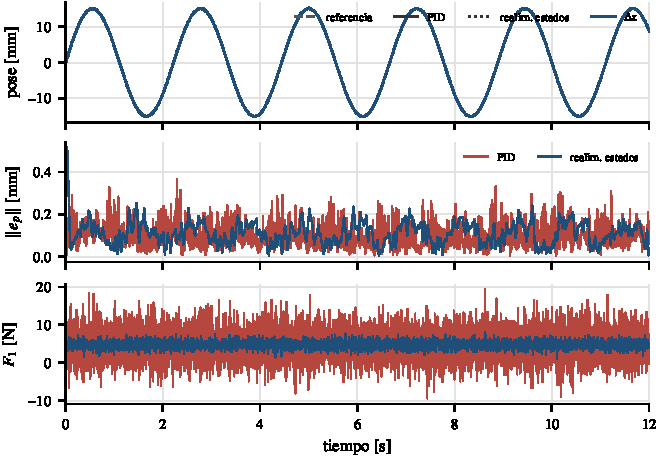
\includegraphics[width=\columnwidth]{ref_sine_z.pdf}
\caption{Senoidal en $z$ (15~mm, 0.45~Hz): referencia, respuesta, norma del error y fuerza de la pata 1.}
\label{fig:refsine}
\end{figure}

\begin{figure}[t]
\centering
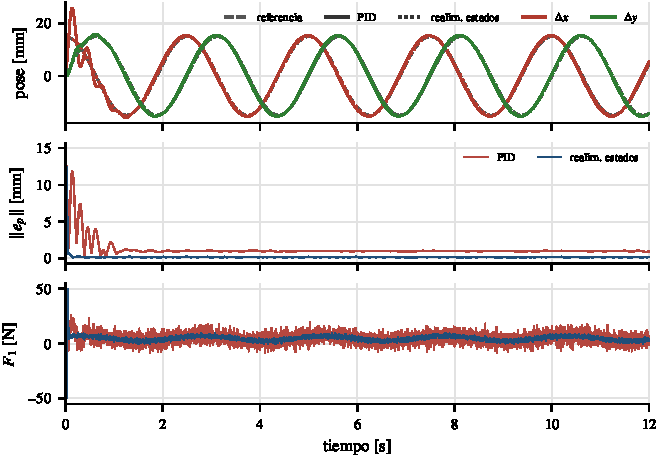
\includegraphics[width=\columnwidth]{ref_circle_3d.pdf}
\caption{Trayectoria circular: referencia, respuesta, norma del error y fuerza de la pata 1.}
\label{fig:refcirc}
\end{figure}

\begin{figure}[t]
\centering
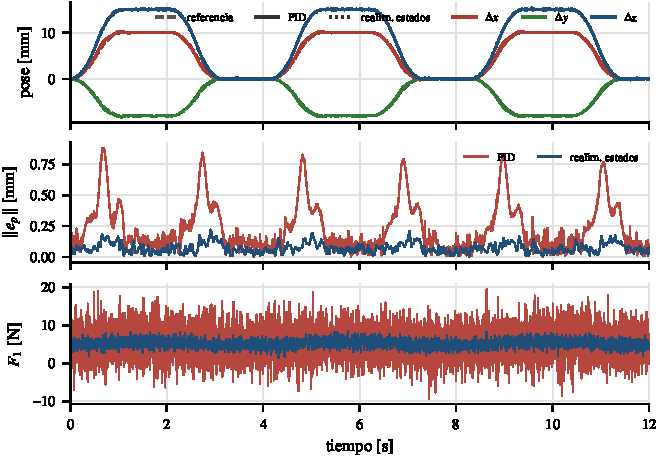
\includegraphics[width=\columnwidth]{ref_min_time.pdf}
\caption{Maniobra de tiempo mínimo (bang-bang) de ida y vuelta: referencia, respuesta, norma del error y fuerza de la pata 1.}
\label{fig:refmin}
\end{figure}

\begin{figure}[t]
\centering
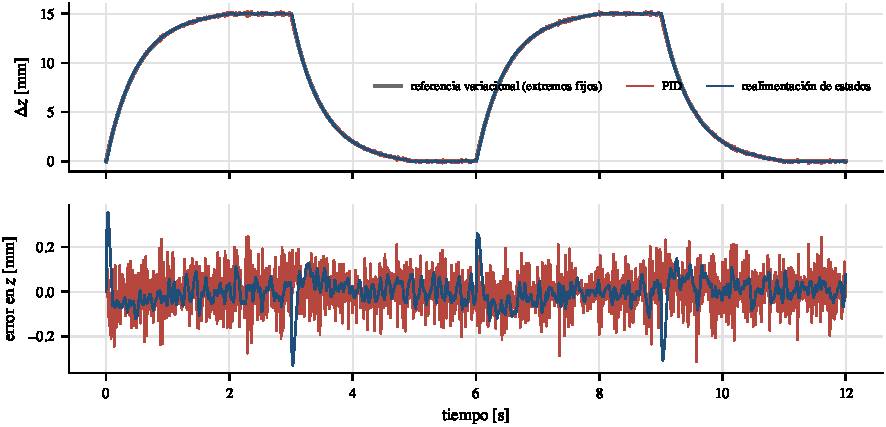
\includegraphics[width=\columnwidth]{seguimiento_variacional.pdf}
\caption{Seguimiento de la trayectoria variacional de extremos fijos~\eqref{eq:fijos} con ambos controladores y error de seguimiento.}
\label{fig:segvar}
\end{figure}

\begin{table*}[t]
\centering
\caption{Índices por tipo de movimiento (planta no lineal, ganancias óptimas, ruido de 0.1 mm, 12 s)}
\label{tab:refind}
\footnotesize
\setlength{\tabcolsep}{4pt}
\begin{tabular}{@{}llrrrrrrr@{}}
\toprule
Referencia & Estrategia & RMS pos [mm] & RMS ang [$^\circ$] & $\|e_p\|_{\max}$ [mm] & ITAE & $J_u$ [N$^2$s] & $|F|_{\max}$ [N] & $F$ sat. [\%] \\
\midrule
\tabinput{tablas/referencias.tex}
\bottomrule
\end{tabular}
\end{table*}

\begin{figure}[t]
\centering
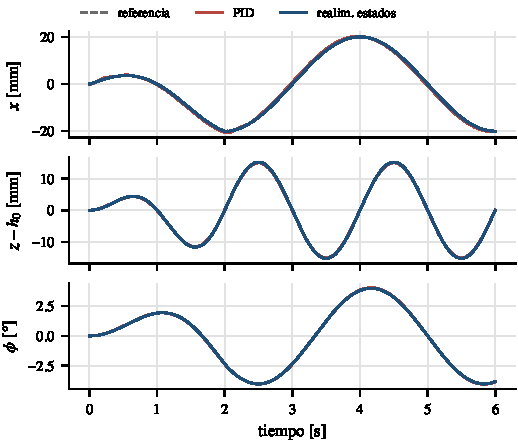
\includegraphics[width=\columnwidth]{banco_6gdl.pdf}
\caption{Maniobra acoplada de 6 GDL sobre la planta no lineal.}
\label{fig:banco}
\end{figure}

% =====================================================================================================
\section{Discusión}\label{sec:discusion}

\textbf{Por qué la realimentación de estados gana en los movimientos acoplados.} La matriz $\vect B_2 = \vect M_0^{-1}\vect J_0\T$ reparte la fuerza de cada pata entre traslación y giro, y $\vect A_{21}$ acopla $x$ con $\theta$ e $y$ con $\phi$ con entradas de 37.9~s$^{-2}$, del mismo orden que la diagonal. El PID ve ese acoplamiento como una perturbación que solo corrige después de producirse; la realimentación de estados lo anticipa porque su ganancia se calcula con el modelo completo. En los movimientos verticales el acoplamiento no se excita y ambas estrategias son equivalentes.

\textbf{Por qué el PID rechaza mejor las perturbaciones.} Su ganancia proporcional, \KpOpt~N/m por pata, es diez veces la cota~\eqref{eq:cotaKp} y responde a la medida de la pata sin pasar por el observador. La realimentación de estados reacciona a través de la estimación, filtrada por un observador lento, y paga con más desviación ante el impulso lo que gana en esfuerzo.

\textbf{El observador lento.} El óptimo resultó con un observador tres veces más lento que el par oscilatorio del controlador, contrario a la regla usual de hacerlo de dos a seis veces más rápido. Con ruido de 0.1~mm y ganancias de posición del orden de $3.8\times10^4$~N/m, un observador rápido transmitiría a cada pata fuerzas de $10^{-4}\cdot3.8\times10^4 = 3.8$~N, comparables con $F_0$. El criterio~\eqref{eq:J}, que penaliza el esfuerzo, prefiere un observador que promedie el ruido: en presencia de ruido, el diseño del observador lo limita la medición y no la velocidad.

\textbf{Limitaciones.} Los resultados provienen de simulación con actuadores ideales de fuerza; la dinámica eléctrica y la fricción de los actuadores reales reducirán los márgenes. Los dos controladores son lineales y se diseñaron en el reposo; en el espacio de trabajo considerado el número de condición del Jacobiano no supera 27.4 y el modelo lineal sigue siendo representativo, pero movimientos más amplios exigirían ganancias programadas o control no lineal. La incertidumbre de masa del 12~\% obtenida en la identificación no se consideró en el diseño; será el punto de partida del control robusto.

% =====================================================================================================
\section{Conclusiones}

La rigidez geométrica negativa de las patas, $F_0/l_0 = 16.8$~N/m por pata, hace inestable la plataforma en lazo abierto, con un polo de 7.62~s$^{-1}$ que duplica cualquier perturbación en 91~ms. En consecuencia, todo control por pata exige una ganancia proporcional mayor que \KlMax~N/m y acción derivativa, sin la cual no existe ganancia estabilizante. Las patas aportan el 28~\% de la inercia de traslación, de modo que un modelo que las omita subestima la masa en casi un tercio; la identificación en lazo cerrado confirma el modelo que las incluye, con masas efectivas dentro del 12~\%.

El error de seguimiento depende de la suavidad de la referencia y no de su rapidez: la maniobra de tiempo mínimo presenta el mismo error que la de extremos fijos, y los mayores errores se concentran en los saltos. Los actuadores operan con holgura, entre 4.8 y 7.4~N en tramos suaves frente al límite de 50~N.

La realimentación de estados con observador de Luenberger es superior en los movimientos acoplados: reduce el error entre 2.5 y 3 veces, con 40~\% menos esfuerzo y menor sensibilidad a la variación de los actuadores. El PID descentralizado rechaza mejor las perturbaciones y es suficiente en los movimientos verticales, con el modelo de una sola pata. Con ruido de medición, el observador óptimo resulta más lento que la parte oscilatoria del controlador. La segunda entrega desarrollará las demás estrategias del proyecto sobre este mismo modelo, protocolo y gemelo digital.

% =====================================================================================================
\begin{thebibliography}{99}
\bibitem{stewart1965} D. Stewart, ``A platform with six degrees of freedom,'' \textit{Proc. Inst. Mech. Eng.}, vol. 180, no. 1, pp. 371--386, 1965.
\bibitem{dasgupta2000} B. Dasgupta and T. S. Mruthyunjaya, ``The Stewart platform manipulator: A review,'' \textit{Mech. Mach. Theory}, vol. 35, no. 1, pp. 15--40, 2000.
\bibitem{merlet2006} J.-P. Merlet, \textit{Parallel Robots}, 2nd ed. Dordrecht: Springer, 2006.
\bibitem{lopes2009} A. M. Lopes, ``Dynamic modeling of a Stewart platform using the generalized momentum approach,'' \textit{Commun. Nonlinear Sci. Numer. Simul.}, vol. 14, no. 8, pp. 3389--3401, 2009.
\bibitem{vanloan1978} C. F. Van Loan, ``Computing integrals involving the matrix exponential,'' \textit{IEEE Trans. Autom. Control}, vol. 23, no. 3, pp. 395--404, 1978.
\bibitem{ljung1999} L. Ljung, \textit{System Identification: Theory for the User}, 2nd ed. Upper Saddle River, NJ: Prentice Hall, 1999.
\bibitem{gelfand1963} I. M. Gelfand and S. V. Fomin, \textit{Calculus of Variations}. Englewood Cliffs, NJ: Prentice Hall, 1963.
\bibitem{kirk1970} D. E. Kirk, \textit{Optimal Control Theory: An Introduction}. Englewood Cliffs, NJ: Prentice Hall, 1970.
\bibitem{moore1976} B. C. Moore, ``On the flexibility offered by state feedback in multivariable systems beyond closed loop eigenvalue assignment,'' \textit{IEEE Trans. Autom. Control}, vol. 21, no. 5, pp. 689--692, 1976.
\bibitem{luenberger1971} D. G. Luenberger, ``An introduction to observers,'' \textit{IEEE Trans. Autom. Control}, vol. 16, no. 6, pp. 596--602, 1971.
\bibitem{franklin1998} G. F. Franklin, J. D. Powell, and M. L. Workman, \textit{Digital Control of Dynamic Systems}, 3rd ed. Menlo Park, CA: Addison-Wesley, 1998.
\bibitem{nelder1965} J. A. Nelder and R. Mead, ``A simplex method for function minimization,'' \textit{Comput. J.}, vol. 7, no. 4, pp. 308--313, 1965.
\end{thebibliography}

\end{document}
